	\chapter[VAE-SNE]{VAE-SNE: a deep generative model for simultaneous dimensionality reduction and clustering \blfootnote{\textbf{Adapted from:} Graving, J. M., & Couzin, I. D. (2020). VAE-SNE: a deep generative model for simultaneous dimensionality reduction and clustering. bioR$\chi$iv, 207993 under a CC-BY-4.0 International License \ccby} \\ \vspace{10mm} \Large Jacob M. Graving, and Iain D. Couzin}
\newpage
\normalsize
\section{Abstract}
Scientific datasets are growing rapidly in scale and complexity. Consequently, the task of understanding these data to answer scientific questions increasingly requires the use of compression algorithms that
reduce dimensionality by combining correlated features and cluster similar observations to summarize
large datasets. Here we introduce a method for both dimension reduction and clustering called
VAE-SNE (variational autoencoder stochastic neighbor embedding). Our model combines elements from
deep learning, probabilistic inference, and manifold learning to produce interpretable compressed
representations while also readily scaling to tens-of-millions of observations. Unlike existing methods,
VAE-SNE simultaneously compresses high-dimensional data and automatically learns a distribution of
clusters within the data — without the need to manually select the number of clusters. This naturally
creates a multi-scale representation, which makes it straightforward to generate coarse-grained
descriptions for large subsets of related observations and select specific regions of interest for further
analysis. VAE-SNE can also quickly and easily embed new samples, detect outliers, and can be optimized
with small batches of data, which makes it possible to compress datasets that are otherwise too large to
fit into memory. We evaluate VAE-SNE as a general purpose method for dimensionality reduction by
applying it to multiple real-world datasets and by comparing its performance with existing methods for
dimensionality reduction. We find that VAE-SNE produces high-quality compressed representations with
results that are on par with existing nonlinear dimensionality reduction algorithms. As a practical
example, we demonstrate how the cluster distribution learned by VAE-SNE can be used for unsupervised
action recognition to detect and classify repeated motifs of stereotyped behavior in high-dimensional
timeseries data. Finally, we also introduce variants of VAE-SNE for embedding data in polar (spherical)
coordinates and for embedding image data from raw pixels. VAE-SNE is a robust, feature-rich, and
scalable method with broad applicability to a range of datasets in the life sciences and beyond.

\section{Introduction}
Modern scientific research generates large, high-resolution datasets that are complex and high-dimensional, where a single observation from an experimental system can contain measurements describing hundreds, or thousands, of features. For example, neuroscientists measure electrical activity across thousands of individual neurons simultaneously \citep{jun2017fully, stringer2019high, stringer2019spontaneous} --- even across the entire brain \citep{ahrens2012brain,ahrens2013whole}; cell biologists and bioinformaticians routinely sequence the transcriptome for thousands of genes across large populations of single cells \citep{samusik2016automated, la2018rna, becht2019dimensionality, linderman2019fast}; behavioral scientists measure the high-dimensional body posture dynamics of animals and humans \citep{stephens2008dimensionality, stephens2011emergence, kain2013leg, berman2014mapping, wiltschko2015mapping, klibaite2017unsupervised, Costa1501, cande2018optogenetic, mathis2018deeplabcut, chambers2019pose, gunel2019deepfly3d, graving2019deepposekit, klibaite2019interacting,
nath2019using,pereira2019fast, bala2020openmonkeystudio, ebbesen2020social, karashchuk2020anipose}; and evolutionary ecologists measure complex morphological patterns across sizeable collections of animal specimens \citep{cuthill2017biology, cuthill2019deep, ezray2019unsupervised, wham2019measuring, zhang2019shell}. While there are many benefits to measuring real-world systems accurately and completely for answering scientific questions, this added complexity poses problems for conventional data analysis methods --- especially those commonly used in the life sciences, like linear models \citep{bolker2009generalized} --- that are designed for small, low-dimensional datasets and typically rely on simplified models with strong, often unrealistic, assumptions for making statistical inferences.

To deal with the complexity of modern data, researchers in many fields have begun to use machine-learning methods known as \textit{dimensionality reduction} and \textit{clustering} to help interpret large, high-dimensional datasets. These algorithms distill correlated features down to a smaller set of components (dimensionality reduction) or group large subsets of observations into a smaller set of classes based on similarity (clustering). Together these methods offer scientists a way to \textit{compress} data, where compression is typically performed with the goal of reducing the size and complexity of a dataset while making only minimal, or very general, a priori assumptions about the true distribution of the data. Because these algorithms derive their compressed representations directly from the structure of the data itself, without human supervision, they are typically known as \textit{unsupervised learning} algorithms. 

Across many scientific disciplines, unsupervised algorithms are rapidly becoming a commonly-used tool for visualizing and interpreting high-dimensional data distributions as well as summarizing large datasets with coarse-grained descriptions and identifying specific subpopulations and regions of interest within the data for further downstream analysis. Researchers have applied these methods to demonstrate how the brain organizes behavior \citep{stephens2008dimensionality, stephens2011emergence, brown2013dictionary, wiltschko2015mapping, berman2016predictability, billings2017instantaneous, cande2018optogenetic, markowitz2018striatum, Costa1501, stringer2019high, stringer2019spontaneous}; describe how cells grow and develop over time \citep{la2018rna}; document new and rare types of cells \citep{grun2015single, linderman2019fast}; gain insights into cancer treatment \citep{tirosh2016dissecting}; and reveal fundamental principles of evolution \citep{cuthill2019deep, ezray2019unsupervised, wham2019measuring}. Therefore, as scientists begin to regularly rely on these algorithms for analyzing complex datasets, the task of ensuring the quality, robustness, and utility of the compressed representations they produce is an issue of considerable importance --- as is the ability to scale these methods to increasingly large datasets.

While existing methods for dimension reduction produce high-quality compressed representations \citep{becht2019dimensionality, kobak2019umap}, they typically lack features for identifying groups of similar data (i.e., learned clusters; but see \citealt{pezzotti2016hierarchical, robinson2020tree}), and despite much progress to improve scalability of existing algorithms \citep{linderman2017efficient, mcinnes2018umap, linderman2019fast}, some of the most widely-used methods are still limited in their ability to scale beyond a few million observations without specialized, high-performance hardware --- especially in the case of large, out-of-core datasets that cannot fit into memory. Recent applications of deep learning \citep{goodfellow2016deep}, and deep generative models in particular (Appendix \ref{appendix:vae}; \citealt{kingma2013vae, rezende2014stochastic}), have begun to address these issues \citep{ding2018scvis, szubert2019ivis, ding2019deep}. Nevertheless, even with the low memory and computational cost of deep learning methods that can be trained with small batches of data on consumer-grade hardware, these new algorithms are still significantly slower to fit to data than more popular methods because they require costly nearest neighbor or pairwise distance calculations \citep{becht2019dimensionality, ding2018scvis, szubert2019ivis}. The majority of these methods also do not provide any built-in mechanism for detecting outliers, which could potentially bias any downstream results and cause statistical errors when testing hypotheses.

There has also been a flurry of recent work on advanced methods for clustering data (e.g., \citealt{campello2013density, jiang2016variational, xie2016unsupervised, guo2017improved, mcinnes2017hdbscan, fogel2019clustering, yang2019deep, robinson2020tree}; and numerous others), including efficient methods that rely on deep learning and deep generative models. However, the vast majority of these methods impose strong assumptions about the shape of the clusters and require the user to manually select the number of clusters fitted to the data --- or, alternatively, involve complex computations that do not scale well to large datasets. Determining how many clusters to fit is typically a non-trivial, unintuitive, and computationally-intensive task for datasets where the number of clusters is not known a priori \citep{milligan1985examination, pham2005selection, fang2012selection, todd2017systematic}. Many recently proposed clustering algorithms are also only evaluated with relatively small ``toy" datasets, such as the MNIST handwritten digit database \citep{lecun2010mnist}, where the data typically have very little noise, no outliers, and the number of clusters is often known a priori. This lack of rigorous real-world assessment casts doubt on the practical utility of these algorithms in cases where datasets have a large number of observations, are naturally noisy or contain outliers, and the number of clusters is unknown, such as those commonly used in the natural sciences.

% Alternatively, some clustering methods rely on non-parametric algorithms that automatically determine the number of clusters from the structure of the data (i.e., local density) and usually make no strong prior assumptions about cluster shape (e.g., \citealt{campello2013density, berman2014mapping, mcinnes2017hdbscan, fogel2019clustering}). Unfortunately, because of these relaxed constraints, non-parametric clustering methods generally do not scale to large datasets as easily as parametric methods, especially in comparison to deep learning methods --- because, as the name suggests, there is no direct parametric mapping between the data and the cluster assignments. This limitation can render non-parametric algorithms difficult to apply to out-of-sample data that were not used for initially optimizing the algorithm. The clustering results produced by non-parametric methods may also be closely comparable to parametric methods in practice \citep{todd2017systematic, fogel2019clustering}, which calls into question the presumed benefits of using these methods in the first place. While dimensionality reduction is typically necessary for applying clustering algorithms to high-dimensional data \citep{parsons2004subspace}, some clustering methods are only tractable for very low-dimensional data (e.g., the watershed clustering algorithm used by \citealt{berman2014mapping}), and this constraint necessitates dramatically reducing the dimensionality of the data to the point that the quality of the final cluster labels is potentially diminished \citep{todd2017systematic}. Some clustering algorithms also require careful tuning of hyperparameters that determine the final clustering configuration, which may be even less intuitive than the task of directly selecting the number of clusters.


Here we aim to address many of the limitations outlined above and unify some of the key methodological concepts from previous work into a single modeling framework. To accomplish this, we introduce a deep generative model for both dimensionality reduction and clustering. We then compare our model with existing methods for dimensionality reduction, and importantly, to ensure that it has practical utility, we demonstrate the application of our method using empirical examples with real-world data from multiple domains. In comparison to existing dimension reduction methods, our proposed method produces low-dimensional data representations with similar, or better, quality while also offering several key improvements. Notably, our approach provides the ability to scale to datasets containing tens-of-millions of observations without specialized, high-performance hardware and automatically learns an interpretable cluster distribution from the data without any manual tuning or expensive computations to determine the number of clusters. Together these results demonstrate that our proposed method is a robust, feature-rich, and scalable tool for data analysis and is widely-applicable to a variety of tasks.

\begin{figure}[!htb]
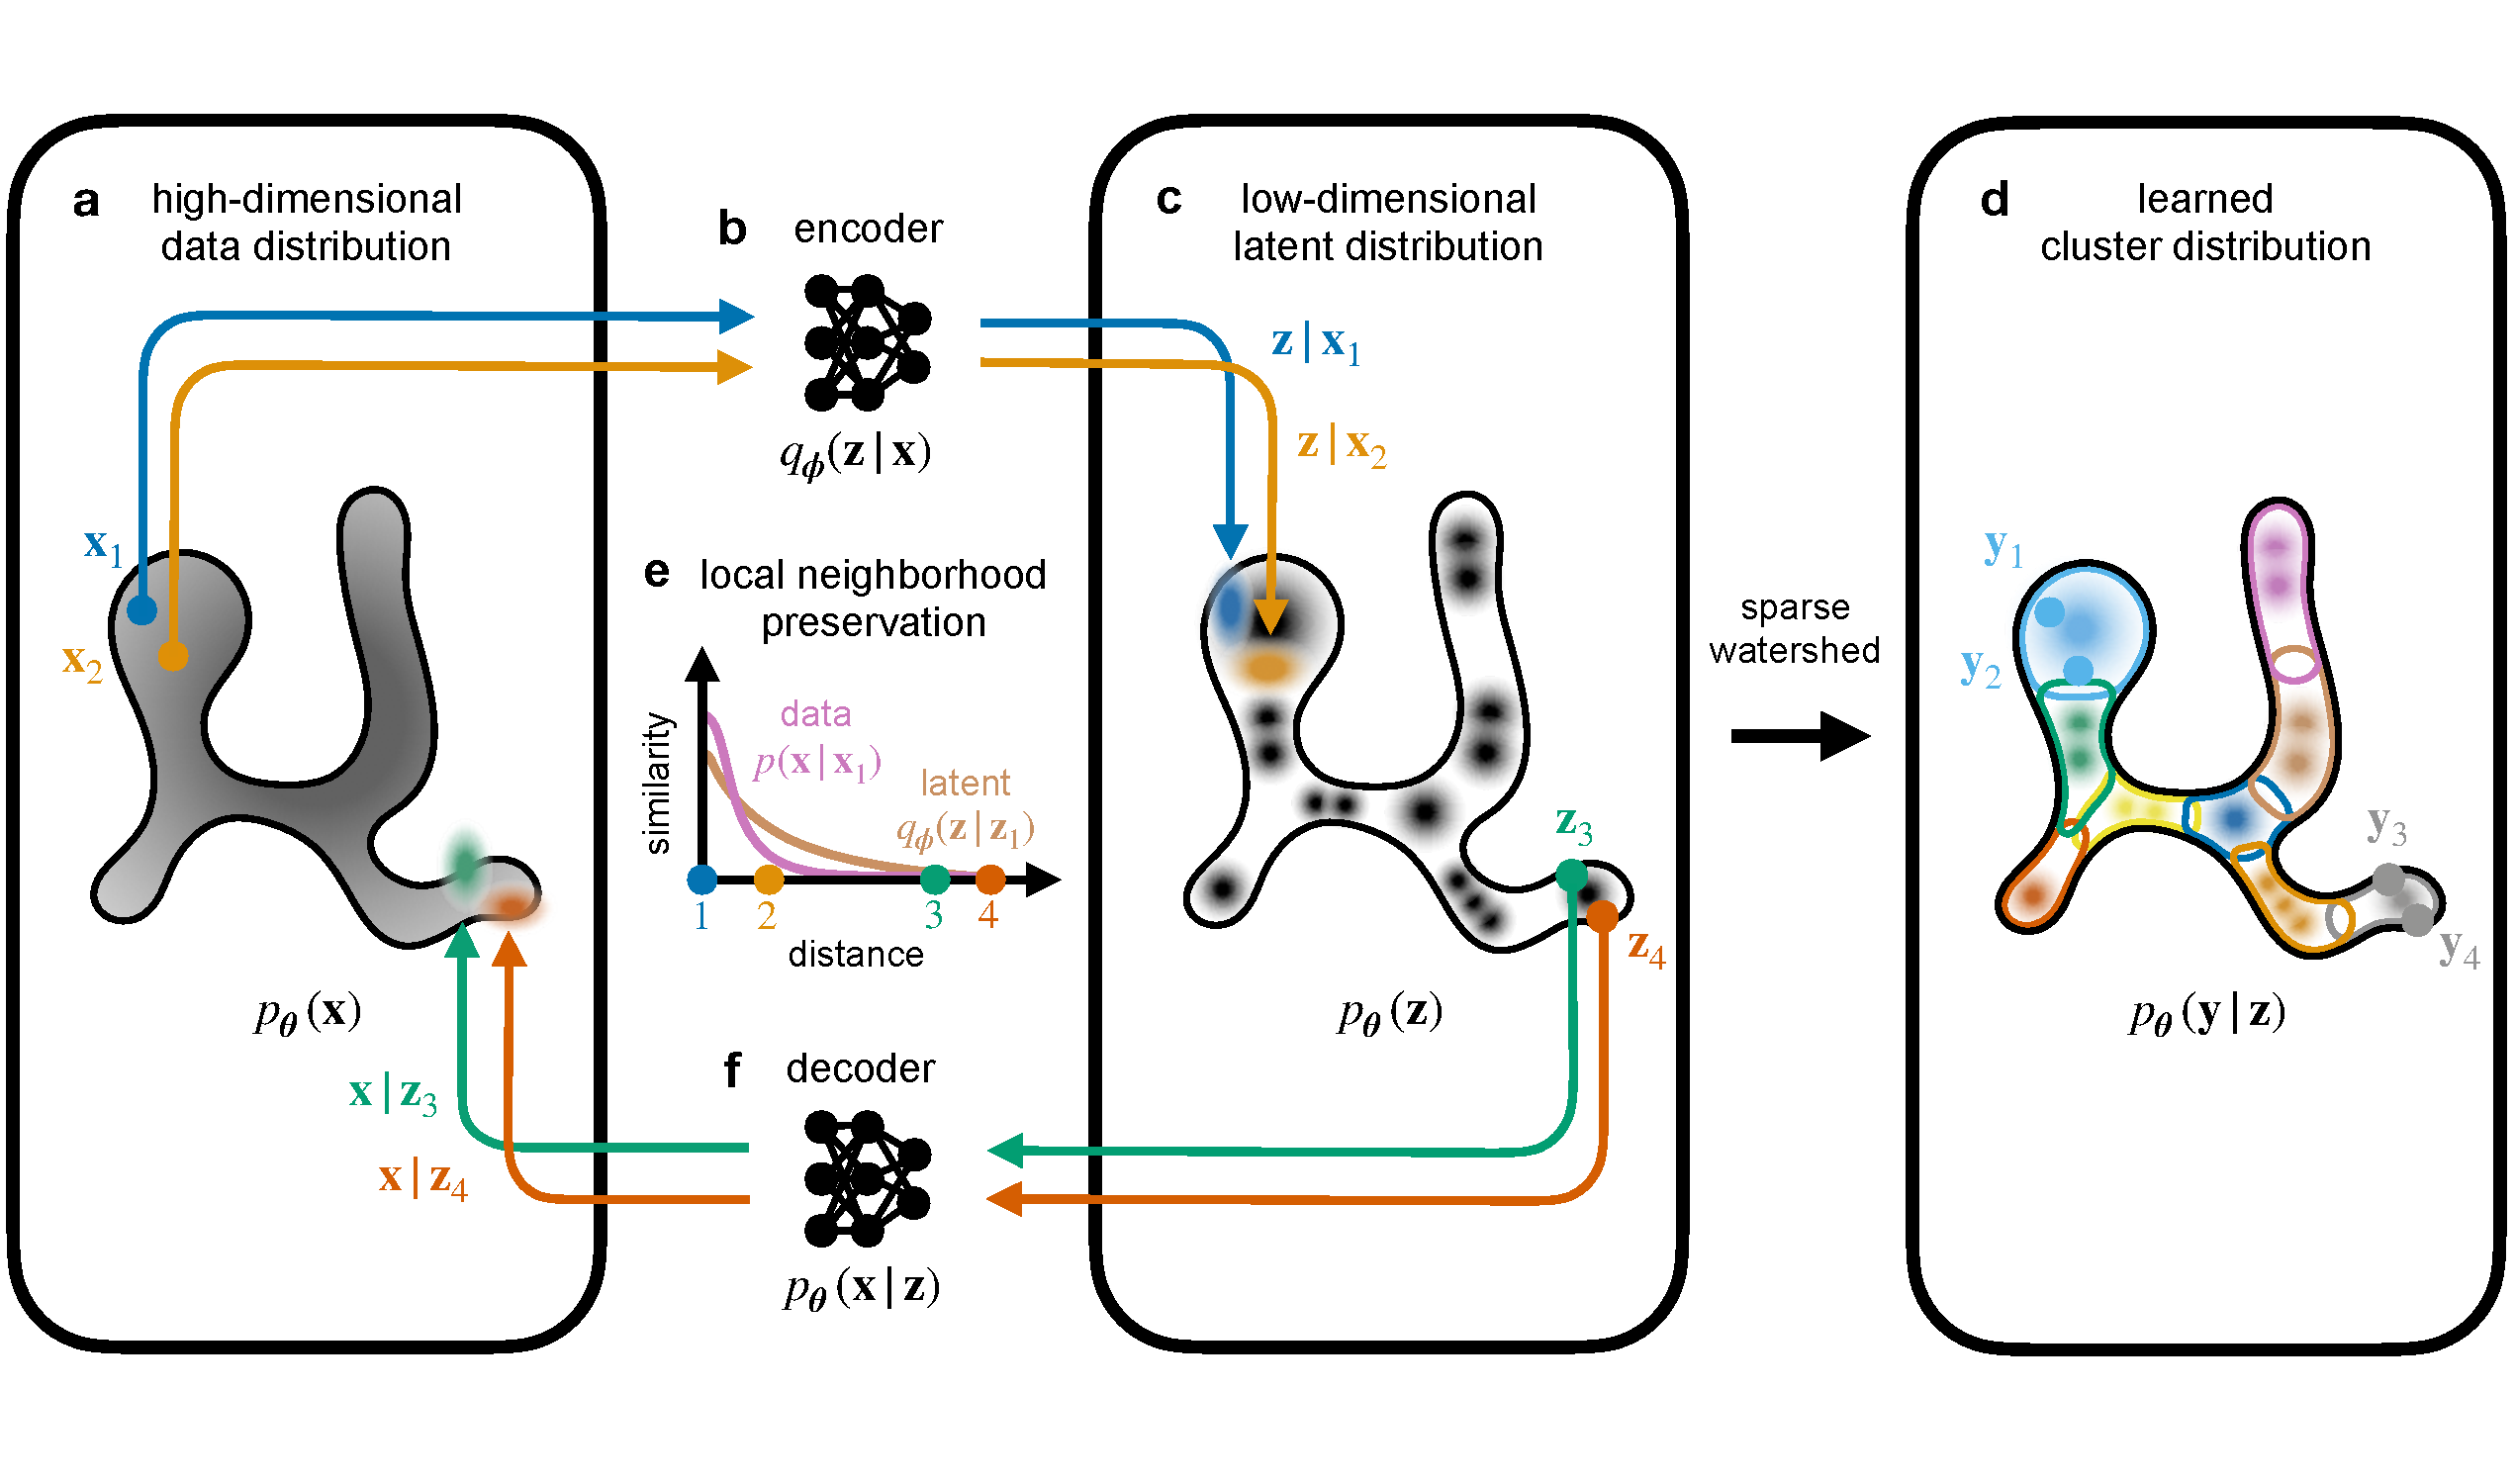
\includegraphics[width=\textwidth]{Graving_IMPRS_Thesis/figures/vaesne_figure.pdf}

\caption{  \textbf{Overview of the VAE-SNE model}. \textbf{a}-\textbf{f}, Observed samples from a high-dimensional data distribution $\mathbf{x} \sim p(\mathbf{x})$ (\textbf{a}) are probabilistically embedded (\textbf{b}) into a low-dimensional latent distribution $p_{\boldsymbol{\theta}}(\mathbf{z})$ (\textbf{c}) using an encoder deep neural network $\mathrm{DNN}_{\boldsymbol{\phi}}: \mathbf{x} \to \mathbf{z}$ to generate an approximate latent posterior distribution $q_{\boldsymbol{\phi}}(\mathbf{z} | \mathbf{x})$. Samples from the latent distribution $\mathbf{z} \sim q_{\boldsymbol{\phi}}(\mathbf{z} | \mathbf{x})$ or $\mathbf{z} \sim p_{\boldsymbol{\theta}}(\mathbf{z})$ (\textbf{c}) are then transformed (\textbf{f}) using a generative decoder deep neural network $\mathrm{DNN}_{\boldsymbol{\theta}}: \mathbf{z} \to \mathbf{x}$ to probabilistically reconstruct the high-dimensional data distribution $p_{\boldsymbol{\theta}}(\mathbf{x} | \mathbf{z})$. Given a set of observed high-dimensional data
$\{\mathbf{x}_1, \mathbf{x}_2, \dots, \mathbf{x}_N\}$ the model parameters for the encoder and decoder $\{\boldsymbol{\theta}, \boldsymbol{\phi}\}$ are optimized so that the approximate posterior for the encoder matches the true posterior from the generative decoder as best as possible, or $q_{\boldsymbol{\phi}}(\mathbf{z} | \mathbf{x}) \approx p_{\boldsymbol{\theta}}(\mathbf{z} | \mathbf{x})$, which then creates a functional mapping between the high-dimensional and low-dimensional distributions. To improve local structure preservation during optimization, pairwise distances between vectors in the high-dimensional and low-dimensional space are optimized using pairwise similarity kernels (\textbf{e}), a probability density function of distance, so that the local neighborhoods around each observation match as best as possible, or $p(\mathbf{x} | \mathbf{x}_i) \approx q_{\boldsymbol{\phi}}(\mathbf{z} | \mathbf{z}_i)$. This preferentially weights the preservation of local neighborhoods over global relationships by assigning more probability mass to nearby neighbors during optimization. The prior for the latent distribution $p_{\boldsymbol{\theta}}(\mathbf{z})$ is also a learned Gaussian mixture distribution (\textbf{c}) that is jointly optimized with the encoder and decoder to fit the observed data and can be used to cluster the latent distribution (\textbf{d}) into a small set of discrete classes $p_{\boldsymbol{\theta}}(\mathbf{y} | \mathbf{z})$ --- where highly-overlapping modes (mixture components) within the distribution are automatically merged into the same class label using sparse watershed assignment (Methods; \citealt{todd2017systematic})}

\label{fig:vaesne_figure} % \label works only AFTER \caption within figure environment

\end{figure}

\section{Results}
We make three main contributions in this paper: (\textbf{1}) First, we introduce a deep generative model for both dimensionality reduction and clustering called variational autoencoder stochastic neighbor embedding (VAE-SNE; Fig. \ref{fig:vaesne_figure}; Methods). VAE-SNE can produce a variety of different compressed representations and readily scales to out-of-core datasets with tens-of-millions of observations. Our model builds on numerous ideas from past work by synthesizing methods from a class of generative models known as variational autoencoders (VAEs; \citealt{kingma2013vae}), the popular dimensionality reduction algorithm (\textit{t}-distributed) stochastic neighbor embedding (SNE/t-SNE;\citealt{hinton2003stochastic, maaten2008tsne}) and its many extensions \citep{van2009ptsne, wang2016vmf, chien2017variational, ding2018scvis}, as well as recent advances in variational inference \citep{kingma2014semi, burda2015iwae, dilokthanakul2016gmvae, cremer2017reinterpreting, tomczak2017vae} and clustering methods \citep{todd2017systematic}. (\textbf{2}) Second, we apply VAE-SNE, and a variety of other popular dimensionality reduction methods, to compress real-world datasets from different domains (Fig. \ref{fig:embedded_data_figure}). We then quantitatively assess how each algorithm performs in preserving important aspects of the data --- including information about local, global, and temporal structure. We also assess generalization to new, out-of-sample data and compare processing speeds for each algorithm. Additionally, we show how the likelihood score produced by VAE-SNE can be used to detect outliers when embedding out-of-sample data. (\textbf{3}) Third, we show how VAE-SNE can be used to automatically cluster large datasets into a small set of interpretable classes. As a practical example, we apply VAE-SNE to a dataset of 21.1 million observations describing the high-dimensional body posture dynamics of a commonly-used model organism --- the fruit fly (\textit{Drosophila melanogaster}) --- to automatically discretize these data into motifs of stereotyped behavior for further analysis (Fig. \ref{fig:cluster_figure}; \citealt{berman2014mapping, pereira2019fast}). These results illustrate how VAE-SNE can be used as a type of automated ethogram for describing the full behavioral repertoire of animals (reviewed by \citealt{anderson2014toward, berman2018measuring, brown2018ethology, datta2019computational}), while also providing several advantages over existing methods for this task.


Our approach (Fig. \ref{fig:vaesne_figure}; Methods) builds on VAEs as a base model for performing dimensionality reduction (Appendix \ref{appendix:vae}), which, like other types of autoencoders \citep{hinton2006reducing}, model high-dimensional data using two deep neural networks: one to encode data to a compressed latent representation, and another to decode the latent vectors and reconstruct the data. However, VAEs are distinct from other autoencoders in that the encoder is used to parameterize continuous distributions of latent vectors --- from which latent vectors are then probabilistically sampled --- rather than embedding each high-dimensional observation as a single point in the latent space. This type of model offers an attractive dimensionality reduction framework because the objective function (Appendix \ref{appendix:elbo}) naturally imparts a trade-off between the complexity of the encoded description and the overall accuracy of the decoded reconstruction \citep{alemi2016deep}. However, these models suffer from multiple long-standing issues including a phenomenon known as \textit{posterior collapse} \citep{alemi2017fixing, dieng2019avoiding} where the latent coordinate space becomes arbitrarily organized and no longer preserves any statistical features of the high-dimensional data distribution. There has been a string of recent work to address these issues including some relatively straightforward solutions \citep{higgins2016beta, dieng2019avoiding} that achieve varying levels of success, as well as new objective functions that involve regularizing the mutual information between the high-dimensional data and latent distribution (e.g., \citealt{zhao2017infovae, rezaabad2019learning}; reviewed by \citealt{poole2019variational}). 

For VAE-SNE, we provide an effective solution to this problem with the addition of a stochastic neighbor regularizer (Appendix \ref{appendix:sne}; \citealt{maaten2008tsne, van2009ptsne, chien2017variational, ding2018scvis}) that optimizes pairwise similarity kernels between the high- and low-dimensional distributions to strengthen local neighborhood preservation and more explicitly retain a useful representation. We also draw on other theoretical and practical improvements from the literature to enhance the performance of VAE-SNE (Methods). For example, we use a Gaussian mixture prior for learning the latent distribution \citep{kingma2014semi, dilokthanakul2016gmvae, tomczak2017vae}. This choice of distribution allows for better local structure preservation and, when combined with sparse watershed assignment to merge overlapping mixture components (Fig. 
\ref{fig:vaesne_figure}; Methods; \citealt{todd2017systematic}), serves as a flexible method for clustering data --- without the need to manually define the number of clusters or impose strong assumptions about cluster shape. We employ several other advances to further improve structure preservation. For instance, we apply a perplexity annealing technique \citep{kobak2019art} to slowly decay the size of the local neighborhoods optimized by the model during training, which helps to preserve structure across multiple scales. Moreover, we extensively optimize the algorithms underlying our model by applying parallel computations on the CPU and GPU that dramatically improve processing speed compared to previous work \citep{ding2018scvis}.

In addition to our three main contributions, we further extend VAE-SNE to demonstrate its flexibility as a framework for dimensionality reduction. To accomplish this, we introduce a von Mises-Fisher variant of VAE-SNE (Appendix \ref{appendix:spherical}; Fig. \ref{fig:spherical_figure}; \ref{fig:spherical_embedding_posture_video}, \ref{fig:spherical_embedding_rna_video}) that embeds data in polar coordinates (rather than Euclidean coordinates) on a 3-D unit sphere, which is potentially a more natural representation for many high-dimensional datasets \citep{davidson2018hyperspherical} and solves the ``crowding" problem common to some methods \citep{maaten2008tsne, ding2019deep}. Finally, we also apply a modified convolutional version of VAE-SNE (Appendix \ref{appendix:conv}; Figs. \ref{fig:shell_figure}, \ref{fig:butterfly_figure}) to visualize natural history images of animal specimen collections \citep{cuthill2019deep, zhang2019shell} by directly embedding the raw pixel data. Our results for these two extensions are described in Appendix \ref{appendix:extensions}.


\subsection{Comparisons with other dimension reduction algorithms}
Current methods for dimensionality reduction generally fall into two classes known as \textit{linear} and \textit{nonlinear} algorithms. Linear algorithms, such as principal components analysis (PCA), compress high-dimensional data by learning linearly weighted combinations (affine transformations) of the original feature set. Typically these algorithms are optimized to preserve the global structure of the data, where local neighborhood relationships are distorted in order to maintain the full coordinate system of the original features as best as possible. On the other hand, nonlinear algorithms (sometimes called manifold learning algorithms) such as t-SNE (\citealt{maaten2008tsne}) and uniform manifold approximation and projection (UMAP; \citealt{mcinnes2018umap}) typically take the opposite approach of prioritizing relative relationships between data points rather than the global coordinate system. This approach allows local neighborhoods to be preserved while potentially sacrificing information about the larger-scale relationships between data points in the global coordinate space --- although, as we demonstrate here, the global distortion imposed by many of these algorithms is actually comparable to that of PCA.

To validate VAE-SNE as a general-purpose method for  dimensionality reduction, we quantitatively compare its performance with other dimension reduction algorithms --- both linear and nonlinear --- using two datasets from different domains (see Methods) describing animal body part dynamics \citep{berman2014mapping, berman2016predictability, pereira2019fast} and single-cell RNA-seq expression profiles for hippocampal neurons \citep{la2018rna}. We benchmark multiple variants of VAE-SNE with different pairwise similarity kernels for preserving local neighborhood information (including kernel functions with learned parameters; Appendix \ref{appendix:sne}), and we compare these results with those from two high-performance variants of t-SNE \citep{maaten2008tsne} known as FIt-SNE \citep{linderman2017efficient, linderman2019fast} and Barnes-Hut-SNE \citep{van2014accelerating}, as well as UMAP \citep{mcinnes2018umap}, and two other deep neural network-based dimension reduction methods: scvis \citep{ding2018scvis}, and ivis \citep{szubert2019ivis}. We also apply PCA in 2, 5, 10, and 100 dimensions for a linear baseline comparison. We fit each algorithm with a training set and also embed an out-of-sample test set to assess generalization to new data. For both the training and test sets, we then quantitatively assess each algorithm's ability to preserve different types of information about the high-dimensional data when compressing the data to two dimensions, including local, global, fine-scale, and temporal information (Methods). We quantify local information preservation for each algorithm by measuring the preservation of both metric (distance- or radius-based) and topological (nearest neighbors-based) neighborhoods that are approximately $1\%$ of the total embedding size; we measure global information preservation by calculating the correlation between pairwise distances in high- and low-dimensional space; we assess fine-scale information by measuring neighborhood preservation for multiple neighborhood sizes $<1\%$ of the total embedding size; and we evaluate temporal information preservation by computing the correlation between high- and low-dimensional temporal derivatives in a timeseries dataset.  Overall the qualitative properties of the embeddings produced by each algorithm are strikingly similar within datasets (Fig. \ref{fig:embedded_data_figure}), which likely indicates shared mathematical properties of how the latent distributions are modeled. However, we do find potentially important quantitative differences between these algorithms in terms of information preservation and processing speed. We summarize our overall assessments of each nonlinear dimension reduction algorithm in Tables \ref{table:info}, \ref{table:speed}, \ref{table:features}.

\begin{figure}[!htb]
\centering
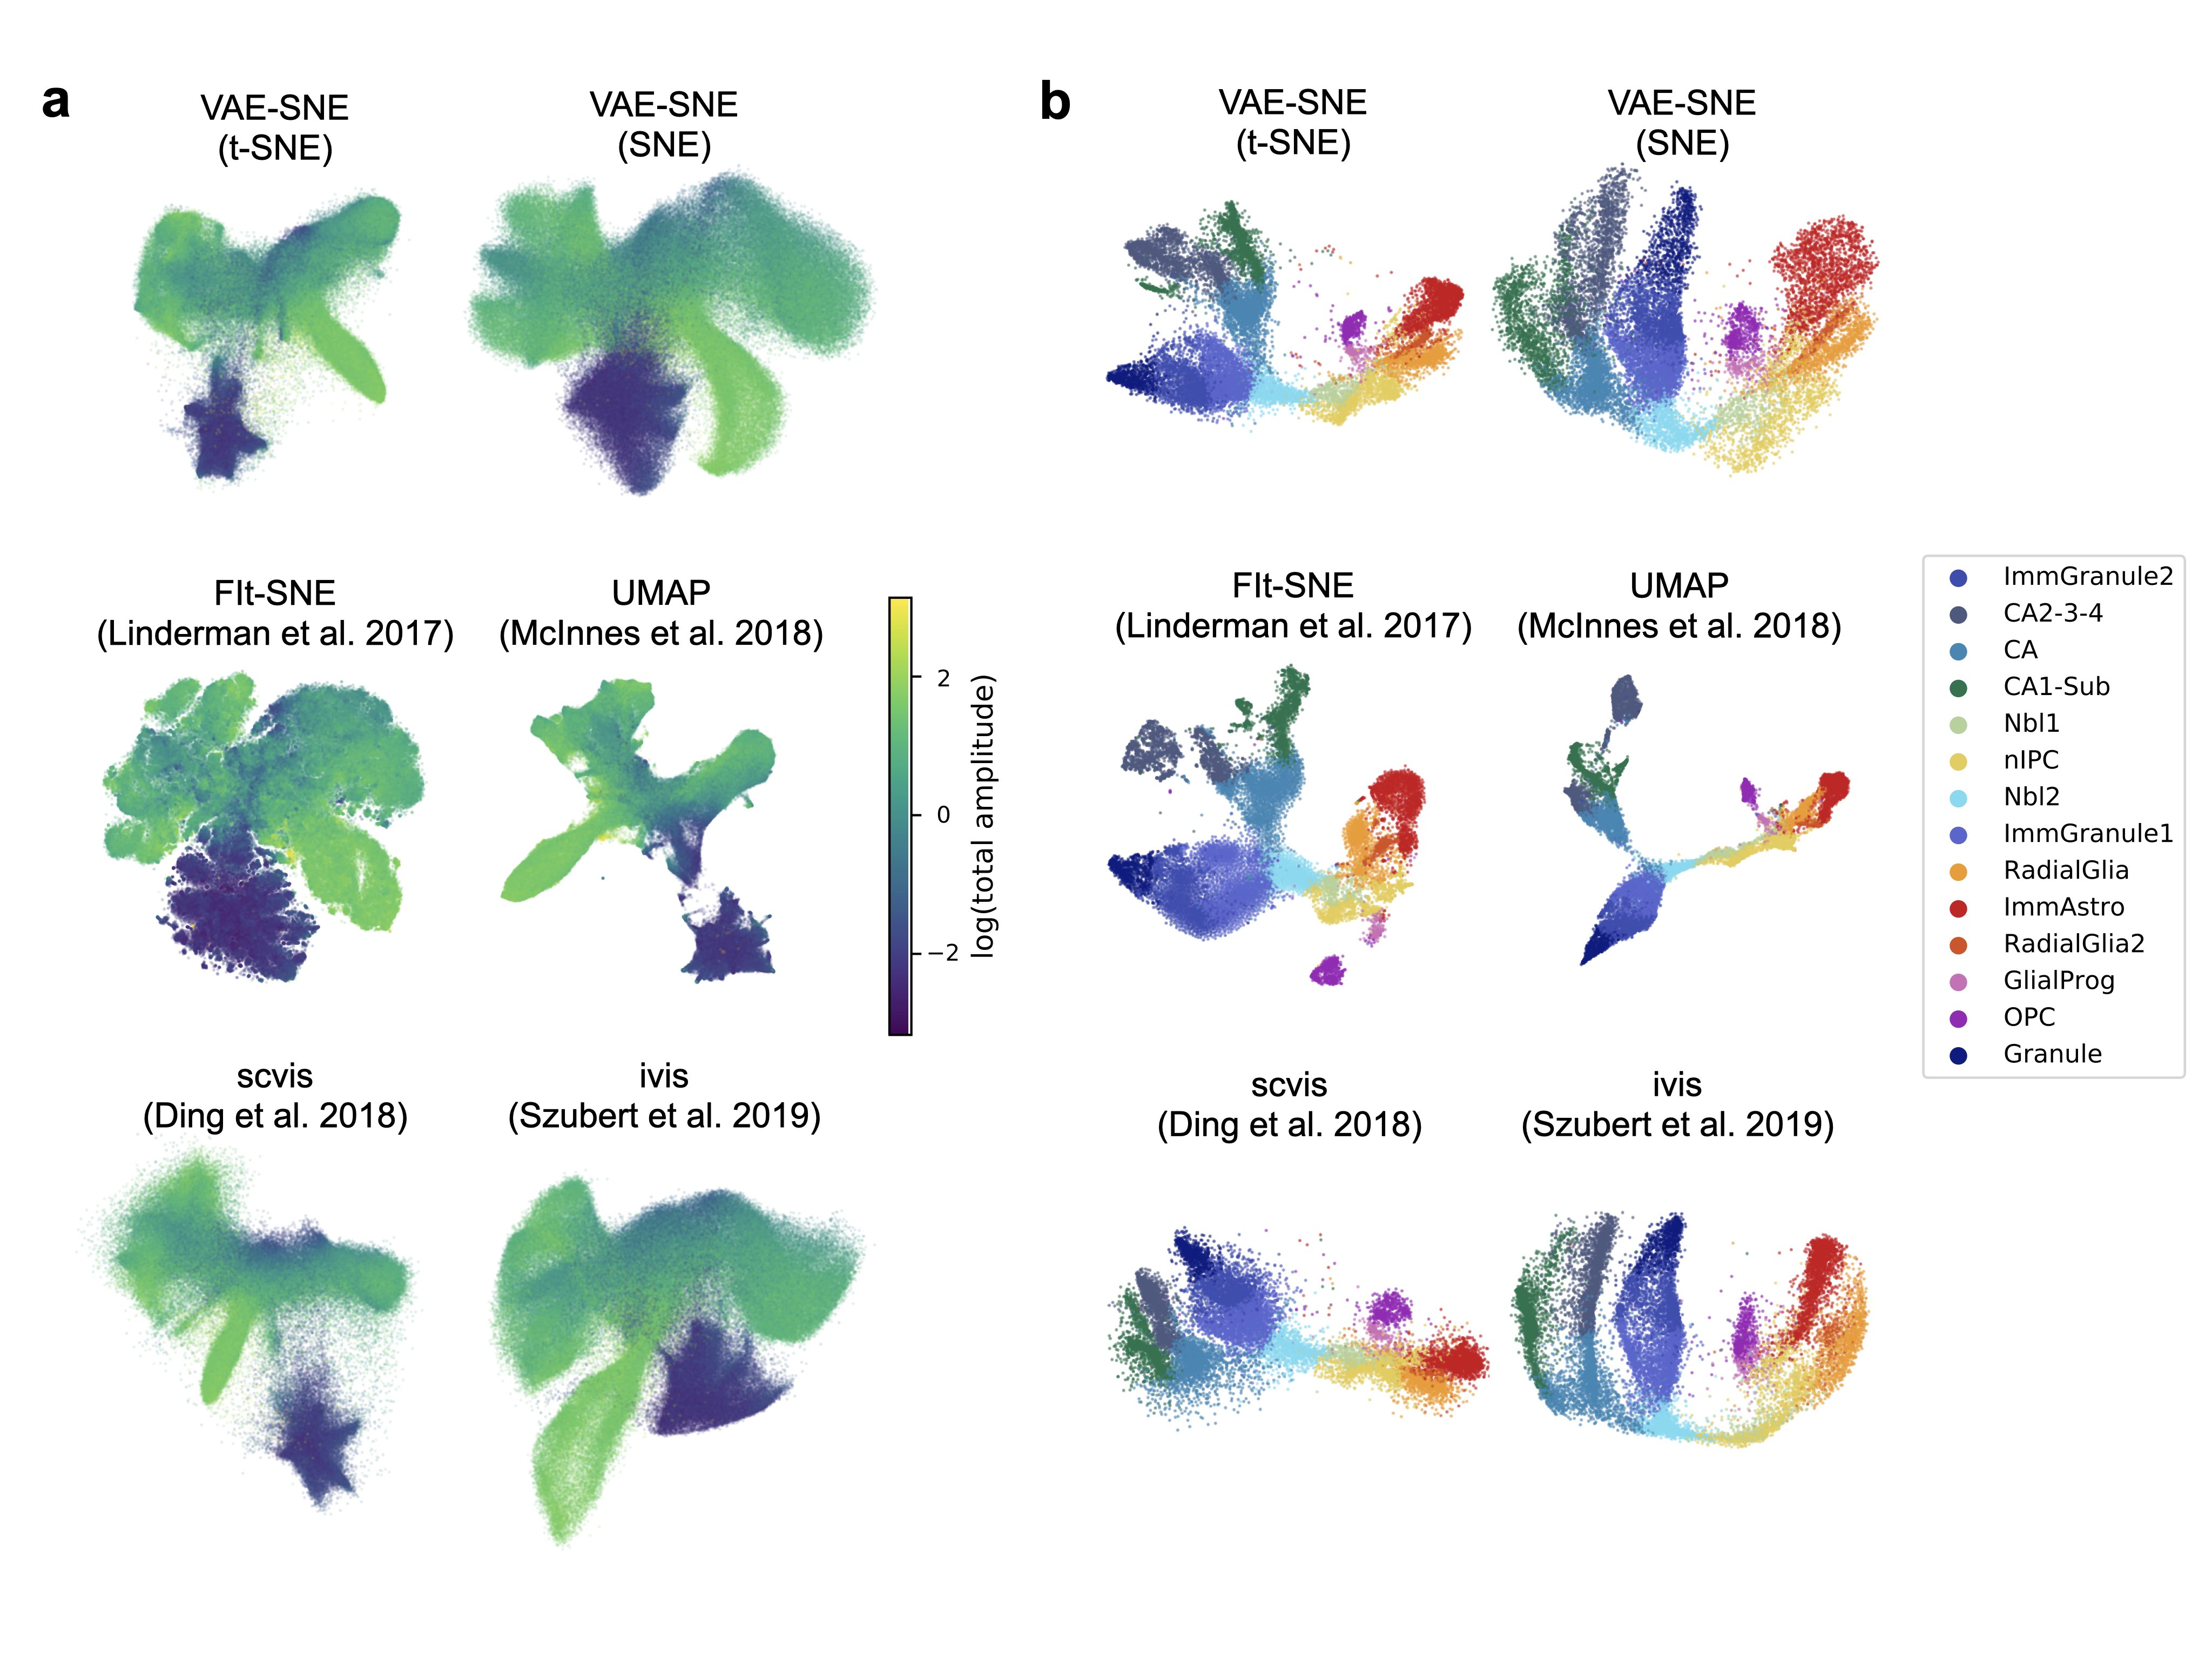
\includegraphics[width=1\textwidth]{Graving_IMPRS_Thesis/figures/embedded_data_figure.jpeg}

\caption{  \textbf{Embeddings for body posture dynamics and single-cell RNA-seq data.} \textbf{a}, 2-D embeddings of body posture dynamics data from \cite{berman2014mapping, berman2016predictability, pereira2019fast} for each algorithm we tested. The color of each point indicates the logarithm of the total amplitude (overall movement) of body parts for each observation. \textbf{b}, 2-D embeddings of single-cell RNA-seq data of developing hippocampal neurons from \cite{la2018rna} for each algorithm. The color of each point indicates the cell type for that observation as described by \cite{la2018rna}.}

\label{fig:embedded_data_figure} % \label works only AFTER \caption within figure environment

\end{figure}

\subsubsection{Local structure preservation}
We find that VAE-SNE compares closely to FIt-SNE \citep{linderman2017efficient}, Barnes-Hut-SNE \citep{van2014accelerating}, and UMAP \citep{mcinnes2018umap} in preserving local structure for both the training set (Figs. \ref{fig:training_set_figure}a, \ref{fig:training_set_appendix_figure}a, \ref{fig:rna_velocity_figure}a) and test set (Figs. \ref{fig:test_set_figure}a, \ref{fig:test_set_appendix_figure}a), while scvis \citep{ding2018scvis} and ivis \citep{szubert2019ivis} perform slightly worse. Our results show that VAE-SNE with a t-SNE similarity kernel \citep{maaten2008tsne} performs the best for preserving local structure, but VAE-SNE with a Gaussian SNE kernel \citep{hinton2003stochastic} also performs well --- similarly to scvis \citep{ding2018scvis} and ivis \citep{szubert2019ivis}. We also find that learning the similarity kernel parameters (for both Gaussian and Student's \textit{t} kernels) as a function of each data point does not improve performance for our local preservation metrics. The top performing algorithms for local structure preservation (VAE-SNE, t-SNE, and UMAP) are closely comparable to 5-dimensional PCA for both metrics we used to assess local neighborhood preservation.

\subsubsection{Global structure preservation}
We find that VAE-SNE also does well in preserving global structure for both the training set (Figs. \ref{fig:training_set_figure}a, \ref{fig:training_set_appendix_figure}b, \ref{fig:rna_velocity_figure}a) and test set (Figs. \ref{fig:test_set_figure}a, \ref{fig:test_set_appendix_figure}b). VAE-SNE with a Gaussian SNE kernel performs best for this metric, but VAE-SNE with a t-SNE kernel also performs nearly as well. Notably all the neural-network-based methods (VAE-SNE, scvis \citealt{ding2018scvis}, ivis \citealt{szubert2019ivis}) outperform both t-SNE and UMAP \citep{mcinnes2018umap} in preserving global structure for both datasets we tested. This is perhaps not surprising given that recent work has shown neural network models tend to learn the same axes as PCA \citep{rolinek2019variational}. Additionally, these results show that learning the similarity kernel parameters as a function of each data point does improve global structure preservation for VAE-SNE with a t-SNE kernel --- likely because it is optimized to be more similar to the Gaussian kernel used to calculate high-dimensional similarities (Appendix \ref{appendix:sne}). The top performing algorithms for this metric are comparable to 2-dimensional PCA, which demonstrates that nonlinear algorithms are capable of preserving the same global information as PCA while also better preserving local structure. On one hand, the scvis \citep{ding2018scvis} algorithm in particular excels at preserving global structure for the single-cell RNA-seq dataset we tested (Fig. \ref{fig:rna_velocity_figure}a), while, on the other hand, ivis \citep{szubert2019ivis} performs much more poorly than the other neural network algorithms for this dataset, and FIt-SNE \citep{linderman2017efficient, linderman2019fast} and Barnes-Hut-SNE \citep{van2014accelerating} perform even worse. We also show that UMAP \citep{mcinnes2018umap} with PCA initialization better preserves global structure than the default Laplacian Eigenmap initialization.

\subsubsection{Fine-scale structure preservation}
In addition to local and global structure preservation, we evaluate the ability of each algorithm to preserve very fine-scale neighborhood information (Figs. \ref{fig:training_set_figure}b, \ref{fig:test_set_figure}b, \ref{fig:rna_velocity_figure}b). We find that both FIt-SNE \citep{linderman2017efficient} and Barnes-Hut-SNE \citep{van2014accelerating} excel at preserving this fine-scale information for the posture dynamics dataset (Figs. \ref{fig:training_set_figure}b, \ref{fig:test_set_figure}b) while every other nonlinear algorithm performs relatively poorly for both the training and test set. For the single-cell RNA-seq dataset, this distinction is not nearly as large and the algorithms all perform more similarly (Fig. \ref{fig:rna_velocity_figure}b), which indicates performance varies depending on the dataset. Performance for the ivis algorithm \citep{szubert2019ivis} is especially poor for this metric on the single cell RNA-seq dataset. However, neighborhood membership for neighborhoods between $1\%$ and $10\%$ of the total embedding size are all similarly well-preserved for each algorithm.

\subsubsection{Temporal structure preservation}
 Because one of the datasets we use for benchmarking is a behavioral timeseries, for these data we also assess the temporal structure preservation of each algorithm (Figs. \ref{fig:test_set_figure}a, \ref{fig:test_set_appendix_figure}c) on the out-of-sample test set (the training set is randomly sampled across multiple timeseries, so temporal information is not preserved). We find that VAE-SNE (particularly the SNE kernel variant), FIt-SNE \citep{linderman2017efficient}, Barnes-Hut-SNE \citep{van2014accelerating}, scvis \citep{ding2018scvis}, and ivis \citep{szubert2019ivis} perform at the same level as 5-dimensional PCA in preserving temporal structure, while UMAP \citep{mcinnes2018umap} performs relatively poorly in comparison to the other algorithms --- even worse than 2-dimensional PCA.

\subsubsection{Speed comparisons}
In addition to assessing information preservation, we also compare the speed the of each algorithm both when fitting the algorithm to the training set (Figs. \ref{fig:training_set_figure}c, \ref{fig:rna_velocity_figure}c) and when embedding an out-of-sample test set (Figs. \ref{fig:test_set_figure}c, \ref{fig:rna_velocity_figure}c). We find that training time increases approximately linearly with the size of the dataset for each algorithm. UMAP \citep{mcinnes2018umap} has the fastest training time (approximately as fast as PCA), followed by FIt-SNE \citep{linderman2017efficient} and Barnes-Hut-SNE \citep{van2014accelerating}, and then VAE-SNE. While VAE-SNE is slower for fitting the training set than both UMAP \citep{mcinnes2018umap} and t-SNE, it is much faster than the other two neural network methods scvis \citep{ding2018scvis} and ivis \citep{szubert2019ivis}. We also demonstrate that VAE-SNE, and the other neural network methods, can quickly embed out-of-sample test data (Figs. \ref{fig:test_set_figure}c, \ref{fig:rna_velocity_figure}c). The time needed for embedding new data is much higher for both t-SNE and UMAP, and while the elapsed time for embedding the test set scales linearly with the number of samples for all algorithms, we also find that it increases with the size of the training set for both UMAP \citep{mcinnes2018umap} and Barnes-Hut-SNE \citep{van2014accelerating}  (Fig. \ref{fig:test_set_figure}c). This is almost certainly because adding new data for these algorithms requires calculating approximate nearest neighbors between the out-of-sample data and the training set, which consequently requires more computation time for larger training sets. Unexpectedly, FIt-SNE \citep{linderman2017efficient} does not exhibit this behavior despite using similar nearest neighbor calculations to Barnes-Hut-SNE \citep{van2014accelerating}. On the other hand, VAE-SNE and other deep learning algorithms do not suffer from this limitation. Finally, while we do not comprehensively assess memory complexity of different algorithms in this paper, we stopped our speed comparisons at data subsets with 232,000 ($\times$ 1500 dimensions) observations because UMAP began to cause out-of-memory errors for larger subsets --- while all of the other algorithms we tested could still successfully run under the same conditions. This helps to illustrate the key advantage of deep learning-based methods, which naturally maintain very low memory complexity by applying optimization using small batches of data.

\subsection{Using the likelihood to assess out-of-sample data}
Because VAE-SNE also calculates a likelihood score for reconstructing the original high-dimensional data, we can use this to assess performance on out-of-sample data, which is an idea originally proposed by \cite{ding2018scvis}. To test this, we calculate the likelihood score for real data from the posture dynamics dataset \citep{berman2014mapping, berman2016predictability, pereira2019fast} and randomly-permuted data (randomized across feature columns) from the same dataset. We find that the likelihood score is reliably lower for the randomized data, and the two likelihood distributions are well separated (Fig. \ref{fig:likelihood_entropy_figure}a), which shows this metric could potentially be used to detect outliers. We also compare the entropy of the approximate posterior distribution for each embedded sample as another potential metric for detecting outliers. While we find that the entropy is much higher for the randomized data, the distribution is highly overlapping with the entropy for the real data (Fig. \ref{fig:likelihood_entropy_figure}b), which indicates the entropy may not be as useful for evaluating the embedding quality.

\begin{figure}[!htb]
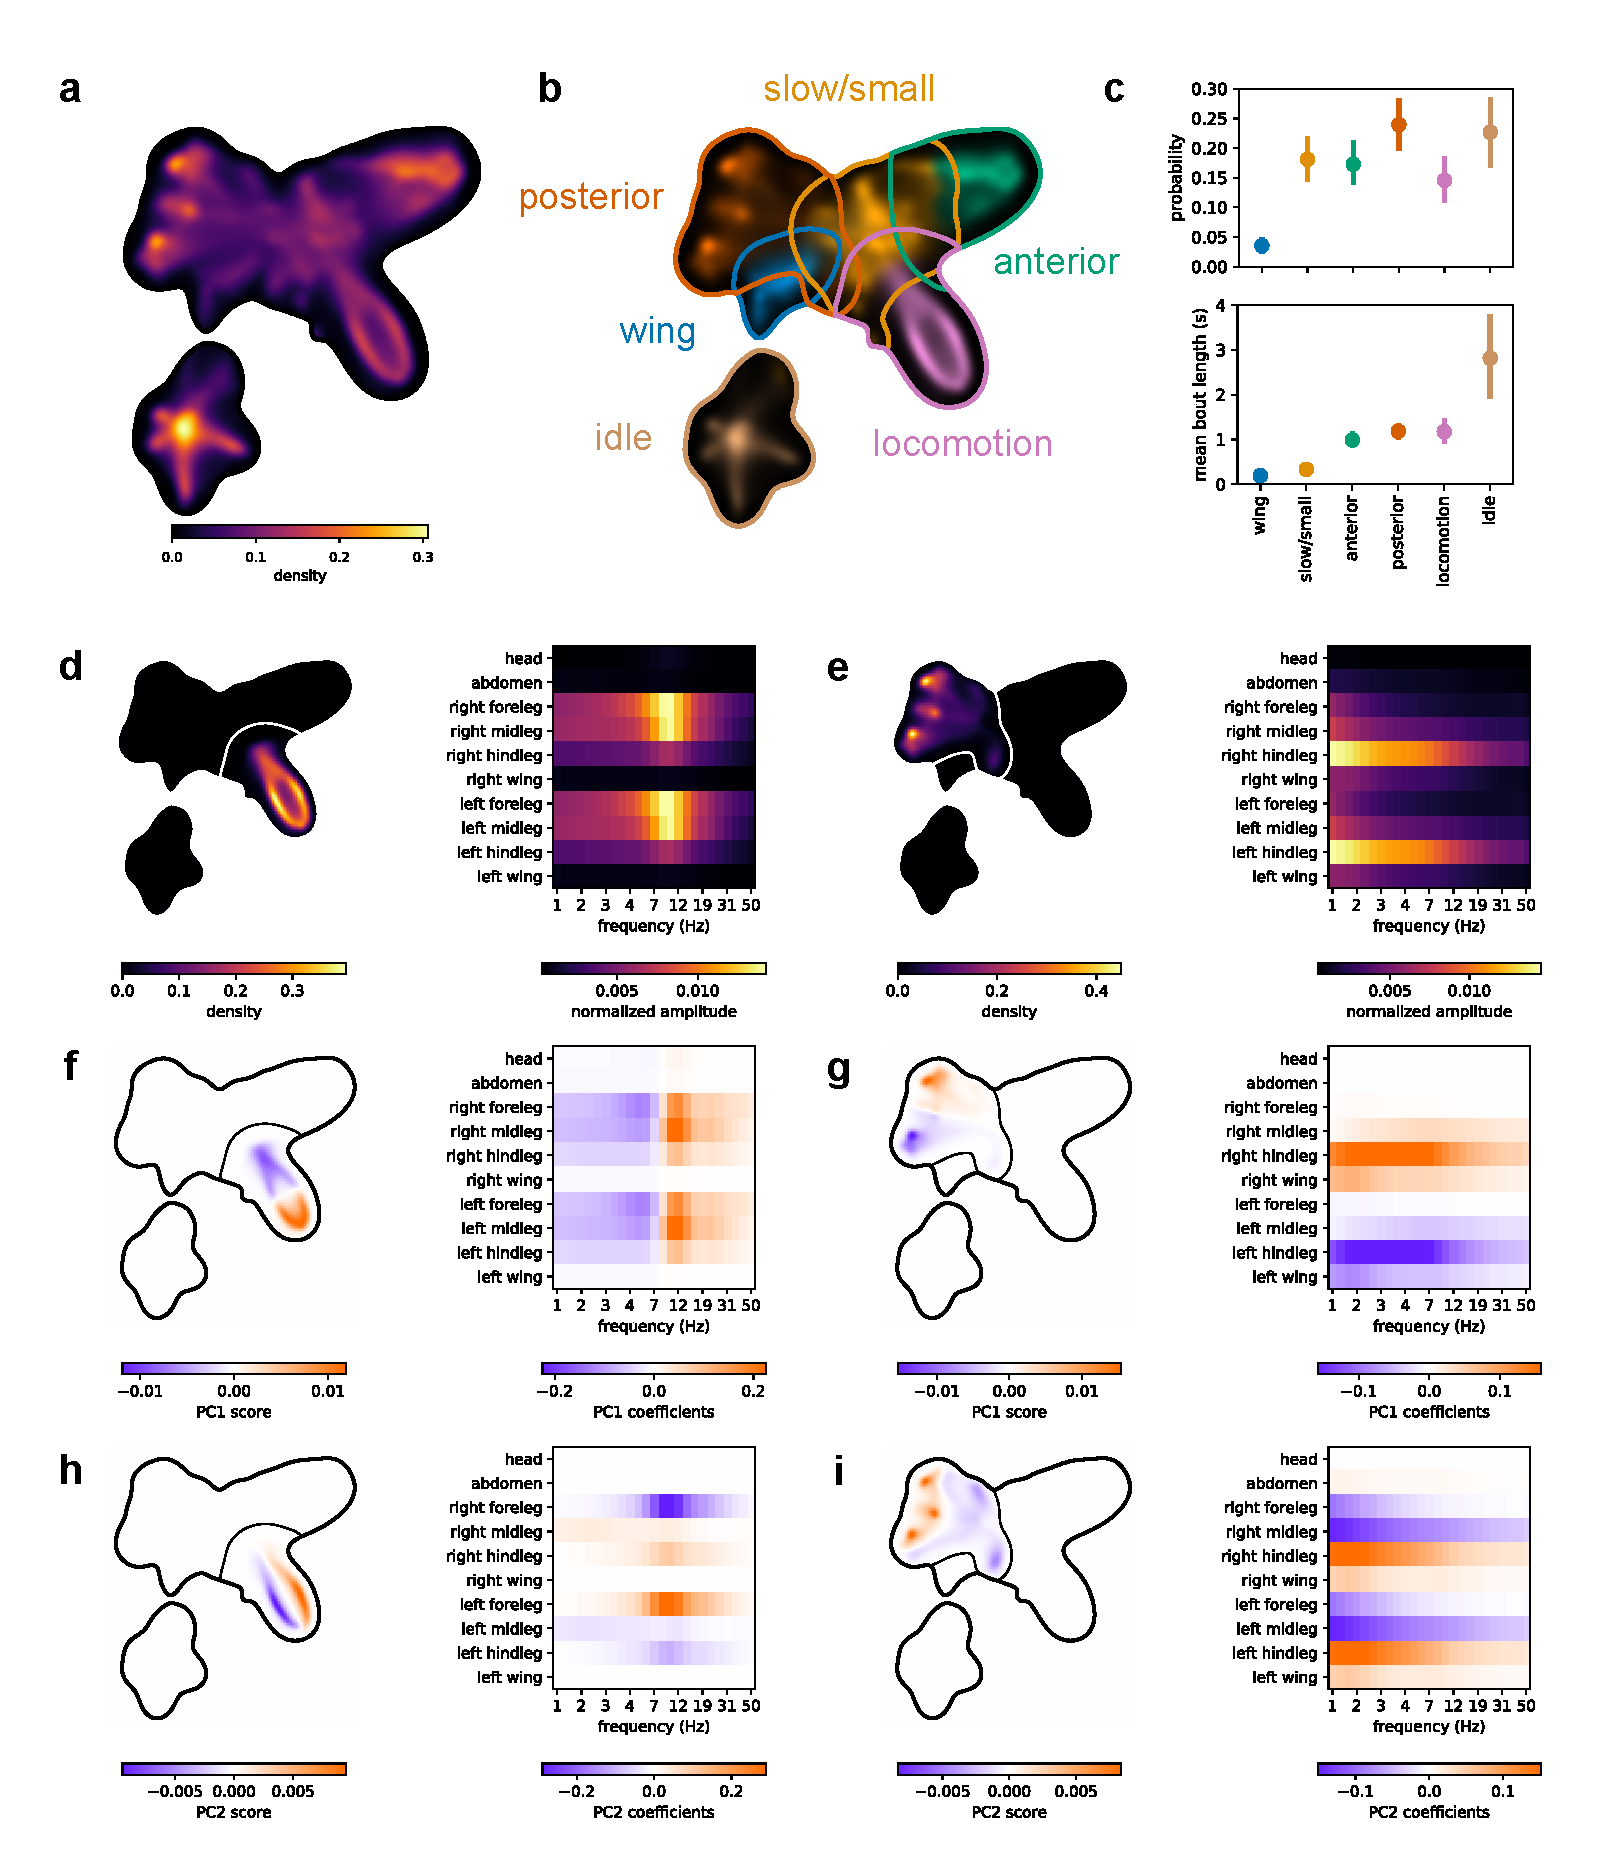
\includegraphics[width=0.9\textwidth]{Graving_IMPRS_Thesis/figures/cluster_figure.pdf}
\centering

\caption{  \textbf{Clustering body posture dynamics.} \textbf{a}, The posterior probability density for the full 21.1 million observation body posture dynamics dataset from \cite{berman2014mapping, berman2016predictability, pereira2019fast} embedded using a 2-dimensional VAE-SNE model. \textbf{b}, The manually-grouped high-level cluster assignments produced using the learned prior from a 30-dimensional VAE-SNE embedding visualized in the 2-D embedding, where contours are the largest 90\% probability density contour for each cluster distribution. \textbf{c}, Mean and 95\% bootstrap intervals of the marginal (stationary) probability and mean bout length for each high-level cluster (n = 59 per cluster). \textbf{d}-\textbf{i}, Visualizations describing the high-level locomotion (\textbf{d},\textbf{f},\textbf{h}; \ref{fig:locomotion_video}; Fig. \ref{fig:locomotion_cluster_figure}) and posterior grooming (\textbf{e},\textbf{g},\textbf{i}; \ref{fig:posterior_video}; Fig. \ref{fig:posterior_cluster_figure}) clusters. \textbf{d-e}, The 2-D posterior probability density for each cluster (left) and the mean spectrogram for each cluster (right). \textbf{f}-\textbf{i}, The principal component scores for the two largest components of the spectrograms assigned to each cluster visualized within the 2-D embedding (left), and the eigenvector coefficients describing the linear contribution of each spectrogram feature (right) for the principal component score.}
\label{fig:cluster_figure}
\end{figure}


\subsection[Clustering body posture dynamics]{Clustering body posture dynamics to reveal stereotyped behavioral organization}
To demonstrate its capabilities as a clustering algorithm, we use VAE-SNE to automatically discretize a dynamical timeseries dataset describing the high-dimensional body posture and behavioral repertoire of 59 freely-behaving fruit flies (\textit{D. melanogaster}; \citealt{berman2014mapping, berman2016predictability, pereira2019fast}) --- a commonly-used model organism for neuroscience, pharmaceutical, and genetics research. To accomplish this, we use the annotated training data from \citep{pereira2019fast} to train a pose estimation model using deep learning-based software (DeepPoseKit; \citealt{graving2019deepposekit}). We then use this trained model to automatically track the spatial locations of 10 body parts (head, legs, wings, abdomen) directly from video timeseries data and generate time-frequency spectrograms describing body-part dynamics for each observation in the timeseries \citep{berman2014mapping}, which naturally incorporates multi-scale temporal information into each data vector. We then apply VAE-SNE to compress the data to a 30-dimensional latent embedding and simultaneously discretize the dynamical posture timeseries into a set of behavioral clusters. We find that, after optimizing the 30-D VAE-SNE model for 5 repeated trials using the full 21.1 million observation dataset and applying sparse watershed assignment to generate cluster labels (Methods; Fig. \ref{fig:vaesne_figure}d; \citealt{todd2017systematic}), VAE-SNE consistently learns a total of 26 low-level behavioral clusters describing distinct, stereotyped body part movements. We also achieve similar (nearly identical) results when clustering in 10-D and 50-D space and when varying the number of components in the Gaussian mixture prior used for clustering --- provided that the number of components is large enough (e.g., $K \geq 100$).

To provide a broad overview of the behavioral structure discovered by VAE-SNE, we manually group these low-level clusters into 6 high-level clusters (Figs. \ref{fig:cluster_figure}, \ref{fig:cluster_appendix_figure}; \ref{fig:sequences_video}) by examining video clips sampled from each cluster (\ref{fig:locomotion_video}--\ref{fig:idle_video}) and by calculating and visualizing the mean spectrograms for each low-level cluster to quantify the average distribution of body part movements across frequencies for each behavioral class (Figs. \ref{fig:locomotion_cluster_figure}d-f, \ref{fig:posterior_cluster_figure}d-i). These high-level clusters include: locomotion (\ref{fig:locomotion_video}), anterior grooming (\ref{fig:anterior_video}), posterior grooming (\ref{fig:posterior_video}), wing movements (\ref{fig:wing_video}), small/slow leg movements (\ref{fig:slow_video}), and idle behavior (\ref{fig:idle_video}). Many of the low-level clusters (10 clusters in total) describe distinct slow/small leg movements, while there are 3 low-level clusters for locomotion (Fig. \ref{fig:locomotion_cluster_figure}), 3 for anterior grooming, 6 for posterior grooming (Fig. \ref{fig:posterior_cluster_figure}), 2 for wing movements, and 2 for idle behavior. Videos and posture timeseries data sampled from each cluster also clearly demonstrate the stereotypy of behaviors within these behavioral classes, which matches well with previous work describing these dynamics \citep{berman2014mapping, berman2016predictability, klibaite2017unsupervised, klibaite2019interacting, pereira2019fast}. Additionally, the principal components of the spectrograms from each high-level cluster (Fig. \ref{fig:cluster_figure}f-i; Fig. \ref{fig:cluster_appendix_figure}d-i) reveal continuous variation related to asymmetrical body movements and differences in peak movement frequency. We calculate basic statistics describing cluster usage across individuals (Figs. \ref{fig:cluster_figure}c, \ref{fig:locomotion_cluster_figure}c, \ref{fig:posterior_cluster_figure}c) including the marginal (stationary) probability of behavioral classes and the mean bout length, or the average amount of time a behavior is performed when an individual transitions into that cluster. In particular, the low probability and short bout length for wing movements and short bout length for slow/small leg movements (Fig. \ref{fig:cluster_figure}c) indicate these clusters may be transitional or idiosyncratic behaviors \citep{todd2017systematic}. For the low-level locomotion clusters (Fig. \ref{fig:locomotion_cluster_figure}) we also calculate the forward component of the leg movement velocity (in body lengths per second, or $\textrm{BL} \cdot \textrm{s}^{-1}$) relative to the egocentric orientation of the animal. We then use the forward velocity to classify each leg in the timeseries as ``swing" (forward velocity $> 0 \, \textrm{BL} \cdot \textrm{s}^{-1}$) or ``stance" (forward velocity $\leq 0 \, \textrm{BL} \cdot \textrm{s}^{-1}$) and find that our low-level locomotion clusters show signatures of distinct locomotory gaits (i.e., tetrapod and tripod gaits; \citealt{mendes2013quantification, pereira2019fast}) with different numbers of legs being used for walking, on average, within each cluster. Together these results demonstrate that VAE-SNE is able to automatically decompose the dynamics of known complex behaviors (\ref{fig:sequences_video}).

Due to the many philosophical complexities of objectively evaluating unsupervised cluster representations (reviewed by \citealt{jain1999data, kleinberg2003impossibility, todd2017systematic}), we forgo any further quantitative assessment of our clustering results and instead leave this for future work. For example, it is unclear how to best select the number of clusters for many different algorithms; how to properly compare algorithms that naturally produce different numbers of clusters and cluster shapes; and what metric(s) should be used to meaningfully evaluate a clustering description as generally ``good" or ``useful" other than manual, qualitative validation of the results, which we already provide here --- though several quantitative descriptors with varying levels of desirability have been recently proposed for behavioral data \citep{todd2017systematic}. Comparing unsupervised cluster labels with a priori-defined labels --- as is common practice (e.g., \citealt{jiang2016variational, xie2016unsupervised, guo2017improved, yang2019deep, luxem2020identifying}) --- is also problematic, as human-supervised descriptions may not accurately capture the underlying structure of the data distribution, and this is especially true for datasets where the goal is to potentially discover subtle differences that are undetectable by humans (e.g., \citealt{wiltschko2015mapping}). Despite the limitations imposed by these complexities, our results still illustrate multiple useful features of VAE-SNE as a general-purpose method.

Overall, we demonstrate how VAE-SNE can be used as a practical, scalable, and flexible tool for clustering real-world high-dimensional data. In this case, we transform posture data into interpretable behavioral labels that are comparable to those from previous methods \citep{berman2014mapping, berman2016predictability, todd2017systematic, klibaite2017unsupervised, cande2018optogenetic, klibaite2019interacting, pereira2019fast}. However, in contrast to many of these existing methods, VAE-SNE performs dimension reduction and clustering simultaneously, and unlike most previously-described algorithms for clustering data (e.g., \citealt{jiang2016variational, xie2016unsupervised, guo2017improved, yang2019deep}), our method learns a small set of decipherable classes without the need to carefully tune the number of clusters fitted to the data, which can often be a non-trivial, unintuitive, and computationally-intensive process \citep{milligan1985examination, pham2005selection, fang2012selection, todd2017systematic}. Instead, any arbitrarily large number will give similar results due to the sparse watershed assignment procedure we use to combine overlapping clusters (Methods; Fig. \ref{fig:vaesne_figure}d; \citealt{todd2017systematic}). 
In contrast to methods that impose strong assumptions about cluster shape, our clustering method has relaxed assumptions and allows for more complex (e.g., non-convex) cluster distributions based on the local structure of the data. 
Additionally, in comparison to prior methods for unsupervised behavioral analysis, VAE-SNE has the advantage of being able to use more than two dimensions for clustering data, which has been shown to provide higher-quality behavioral labels with many potentially-desirable properties \citep{todd2017systematic}. Finally, our results further show that there is no need to carefully select a subset of data to use for training (e.g., the importance sampling technique described by \citealt{berman2014mapping}), which can also be a time-consuming process. Instead, VAE-SNE can be readily applied to large datasets that cannot fit into memory while still successfully detecting relatively short-lived and infrequent types of behavior, such as wing movements (Fig. \ref{fig:cluster_figure}b-c; \ref{fig:wing_video}).

\section{Discussion}
Here we introduce VAE-SNE, a deep generative model for simultaneously reducing dimensionality and clustering data. We compare VAE-SNE to existing methods for dimensionality reduction and demonstrate its utility and versatility using real-world examples. Our results establish that VAE-SNE is able to generate robust and interpretable compressed representations for data from different domains and is comparable in performance to other nonlinear methods for dimensionality reduction. In contrast to these existing methods, VAE-SNE has the advantage of being able to automatically cluster similar observations into a small set of classes, which can then be used to summarize large datasets with coarse-grained descriptors or select specific subpopulations of data for more detailed analysis. Our approach can also readily scale to very large datasets by leveraging techniques from deep learning --- including, and especially, out-of-core data that cannot fit into memory. However, despite these strengths, VAE-SNE still has important limitations depending on the goals of the user, and there are many ways in which the model could be improved or extended in subsequent iterations. There are also other domains that VAE-SNE could be applied to in the future.

VAE-SNE preserves local relationships while also minimizing global structure distortion. Additionally, while VAE-SNE is not explicitly an autoregressive model, it still preserves a good deal of high-dimensional timeseries information. However, our results also show that VAE-SNE, and most of the other dimension reduction methods we tested, does not accurately preserve fine-scale structure (neighborhoods $<$1\% of the total embedding size). For many applications, preserving these details may be unimportant, but this structure has been shown to be useful for detecting infrequent types of data, such as rare cell types \citep{linderman2019fast}. Therefore, our results suggest that if researchers wish to preserve this type of information they should use FIt-SNE \citep{linderman2017efficient, linderman2019fast} or Barnes-Hut-SNE \citep{van2014accelerating} over other algorithms for dimension reduction. We also find that, when initialized with PCA over the default initialization, UMAP \citep{mcinnes2018umap} preserves global structure slightly better without noticeably affecting local structure preservation, so PCA may be a more advantageous choice for initializing UMAP embeddings.

VAE-SNE optimizes faster than existing deep learning methods for dimensionality reduction, but FIt-SNE \citep{linderman2017efficient, linderman2019fast}, Barnes-Hut-SNE \citep{van2014accelerating}, and UMAP \citep{mcinnes2018umap} are still faster. However, the training time for deep-neural-network methods like VAE-SNE and ivis \citep{szubert2019ivis} can be variable due to the use of early stopping criteria that automatically end training when no improvement in the objective function is detected. These early stopping criteria could be easily adjusted to further shorten (or lengthen) training time. While we did not assess performance during the optimization process, much of the training time for VAE-SNE is spent on minor improvements to the objective function, which indicates adequate results can also be achieved with less training time. Additionally, FIt-SNE \citep{linderman2017efficient, linderman2019fast}, Barnes-Hut-SNE \citep{van2014accelerating}, and UMAP \citep{mcinnes2018umap}, are much slower for embedding new data because they calculate nearest neighbors for the new data and further optimize the embedding, which VAE-SNE does not require due to its learned encoder function. For smaller datasets that can fit in memory FIt-SNE \citep{linderman2017efficient, linderman2019fast}, Barnes-Hut-SNE \citep{van2014accelerating}, and UMAP \citep{mcinnes2018umap} are still attractive options for dimensionality reduction, but for datasets that do no fit into memory, VAE-SNE provides some distinct advantages.

VAE-SNE has the ability to detect outliers and assess the embedding quality for out-of-sample data. This provides a straightforward mechanism for identifying new data to include in the training set, which can further improve performance. Most of the other algorithms we tested, or at least the specific software implementations we tested, provide no mechanism for quantitatively assessing embedding quality for each observation --- with outliers being simply embedded under the assumption that the data are well supported by the training distribution. This can cause problems for any downstream analysis, especially when using statistical tests to answer scientific questions. Further improvements for outlier detection might include the use of Bayesian inference \citep{hafner2018reliable} or other methods for estimating predictive uncertainty (reviewed by \citealt{kendall2017uncertainties}). 

We demonstrate that results produced by VAE-SNE can serve as a highly-interpretable coarse-grained description of tens-of-millions of observations --- with several advantages over existing methods for clustering data. Applying VAE-SNE to future research in the behavioral sciences could help to reveal the genetic, environmental, and neural underpinnings of animal behavior \citep{berman2018measuring, brown2018ethology, datta2019computational} --- especially when combined with recent advances in behavioral measurement \citep{mathis2018deeplabcut, pereira2019fast, graving2019deepposekit, gunel2019deepfly3d} as well as genetic \citep{ran2013genome,doudna2014new}, sensory \citep{stowers2017virtual}, and neural \citep{bath2014flymad, cande2018optogenetic} manipulations. The clustering capabilities of VAE-SNE could also be applied to other types of data, such as single-cell RNA-seq data \citep{ding2018scvis, la2018rna} and natural history images \citep{cuthill2019deep, zhang2019shell}, but we leave this as future work for other researchers and domain experts to explore and validate. VAE-SNE might also be further improved by the use of more complex hierarchical clustering distributions \citep{tomczak2017vae, roberts2018hierarchical, razavi2019generating}, where additional scales with finer- or coarser-grained descriptions can be selected from the model for post-hoc analysis. Recent work has also shown that iteratively adjusting the parameters of the t-SNE similarity kernel can be used to generate a hierarchy of clusters in the latent embedding \citep{robinson2020tree}, which could be potentially applied to VAE-SNE as well.

To demonstrate the flexibility of VAE-SNE as a deep learning model, we introduce a variant for embedding data in polar coordinates on a unit sphere (Appendix \ref{appendix:spherical}). We find that VAE-SNE successfully preserves structure in a spherical embedding as well (Fig. \ref{fig:spherical_figure}; \ref{fig:spherical_embedding_posture_video}; \ref{fig:spherical_embedding_rna_video}), which may be a more natural way to model some high-dimensional data sets \citep{davidson2018hyperspherical} since it avoids the ``crowding" problem common to other embedding methods \citep{maaten2008tsne, ding2019deep}. While we focus on the Euclidean and cosine distances for calculating local neighborhoods, any differentiable distance function could potentially be substituted to create different embedding geometries, and, while we focus on kernels from the location-scale family of probability distributions (i.e. Gaussian, Student's \textit{t}), other log probability functions could potentially be used as well.

We also introduce a convolutional version of VAE-SNE for embedding images directly from raw pixel data (Appendix \ref{appendix:conv}). After applying this model to natural history images, we find that it groups perceptually-similar images based on complex sets of image features that correspond with taxonomic groupings (Figs. \ref{fig:shell_figure}, \ref{fig:butterfly_figure}). These results indicate that convolutional VAE-SNE may be useful for tasks such as relating distributions of complex animal coloration patterns to ecological, evolutionary, and behavioral function \citep{cuthill2017biology, cuthill2019deep, ezray2019unsupervised, wham2019measuring}. Future applications might include applying VAE-SNE to audio data (e.g., \citealt{oord2016wavenet, sainburg2019latent}).

There are multitude of ways in which VAE-SNE could be further improved or extended. Naturally, future work could apply more recent advances in variational and probabilistic inference like normalizing flows \citep{rezende2015variational, kingma2016improved, papamakarios2017masked}, which allow data to be modeled with a more direct invertible mapping from the latent posterior to the data distribution, while also employing flexible, arbitrarily-complex distributions. The latent distribution used for VAE-SNE could also be modeled using many other types of representations such as quantized \citep{van2017neural} or categorical \citep{jang2016categorical, maddison2016concrete} distributions. Recent progress in generative adversarial networks (GANs; \citealt{goodfellow2014generative}), may also provide further enhancements for modeling complex feature dependencies within the data distribution \citep{larsen2016autoencoding,srivastava2017veegan, dieng2019prescribed}. Timeseries data could be explicitly modeled using autoregressive deep neural networks (e.g., \citealt{oord2016wavenet}) for the encoder and decoder similar to \cite{wiltschko2015mapping, johnson2016composing, sussillo2016lfads, markowitz2018striatum, pandarinath2018lfads, luxem2020identifying}, and the latent distribution can be optimized to accurately predict future observations, which has been shown to be a useful framework for modeling behavior \citep{berman2016predictability, luxem2020identifying}. Additionally, computational efficiency might be further improved by applying recent advances in metric \citep{sohn2016improved} and contrastive learning \citep{chen2020simple}, which may reduce or eliminate the need to perform expensive pairwise computations. Recent work on density-preserving versions of t-SNE and UMAP \citep{narayan2020density} could also be incorporated to further improve the embedding quality.

Explicitly modeling hierarchical structure caused by variance across individual trials and subjects \citep{pandarinath2018lfads} and batch effects due to variance in sampling procedures \citep{ding2019deep} is also important for improving VAE-SNE in the future. These effects could be accounted for with more complex, hierarchically-parameterized models \citep{sussillo2016lfads, pandarinath2018lfads}, hierarchical latent distributions \citep{tomczak2017vae, roberts2018hierarchical, razavi2019generating}, and new similarity kernels --- such as the conditional t-SNE kernel recently proposed by \cite{kang2019conditional}. The general use of conditional (e.g., \citealt{van2016conditional}) or supervised (e.g., \citealt{alemi2016deep}) labels when optimizing the model could also help to integrate additional prior information about the data distribution into the latent distribution, the latter of which is already a feature of both UMAP \citep{mcinnes2018umap} and ivis \citep{szubert2019ivis}. 

In summary, VAE-SNE is a general-purpose deep learning model for both dimension reduction and clustering that can be applied to many different types of data and readily scales to large datasets. Together our results illustrate that it is a robust, feature-rich method with multiple distinct advantages that make it an effective tool for analyzing real-world datasets across disciplines.

\section{Methods}

\subsection{The VAE-SNE model}

VAE-SNE is a variational autoencoder (VAE; Appendix \ref{appendix:vae}) with a learned Gaussian mixture prior \citep{kingma2014semi, dilokthanakul2016gmvae, tomczak2017vae} that is optimized using the $\mathrm{ELBO}$ objective function (derived in Appendix \ref{appendix:elbo}) with an additional local neighborhood regularizer \citep{hinton2003stochastic, maaten2008tsne, van2009ptsne, ding2018scvis}. The likelihood and divergence terms from the $\mathrm{ELBO}$ objective can be broadly considered as an information theoretic trade-off between reconstruction accuracy (distortion) and compression (rate) respectively \citep{alemi2016deep, chalk2016relevant, alemi2017fixing}, which makes VAEs an attractive solution for dimensionality reduction. However, there are implicit problems with the $\mathrm{ELBO}$ objective (reviewed by \citealt{alemi2017fixing, dieng2019avoiding}) that may prevent the model from learning a useful latent representation --- e.g., a powerful, overparameterized decoder can simply ignore the compressed latent codes but still produce high-quality reconstructions. These issues render VAEs problematic as a general method for reducing dimensionality, as the primary purpose of dimensionality reduction is to create compressed representations that preserve important statistical features of the original data distribution. 

\subsubsection{Regularizing the ELBO to improve structure preservation}
We address the problems outlined above by optimizing VAE-SNE with a regularized version of the $\mathrm{ELBO}$. This modification introduces a pairwise similarity regularizer derived from the (\textit{t}-distributed) stochastic neighbor embedding (SNE/t-SNE) objective \citep{hinton2003stochastic, maaten2008tsne, van2009ptsne}. This idea of using the SNE objective for regularizing the latent space of VAEs was first proposed by \cite{chien2017variational}, which they called variational manifold probabilistic linear discriminant analysis (vm-PLDA), and later independently proposed by \cite{ding2018scvis} with their scvis model. However, the idea of applying the SNE objective to autoencoders, and deep neural networks in general, was introduced much earlier by \cite{van2009ptsne} with parametric t-SNE (pt-SNE), who proposed to use this objective in conjunction with an autoencoder to jointly learn a latent embedding. The pt-SNE model \citep{van2009ptsne} was also recently combined with advances from the Barnes-Hut-SNE algorithm \citep{van2014accelerating} under the name net-SNE \citep{cho2018generalizable}. Additionally, \cite{moody2017vtsne} developed one of the first publicly-available pieces of software to combine the SNE objective with variational inference (variational t-SNE, or vt-SNE; and topic-SNE) but did not use a deep neural network to amortize inference across a set of shared parameters. \cite{im2018stochastic} also proposed a variational bound on the t-SNE objective to improve optimization.

Here we apply the SNE objective to a VAE in a similar fashion to \cite{ding2018scvis}. That is, we use the SNE objective as a method of better preserving structure in the latent embedding produced by our VAE, which improves the usefulness of the compressed representation (approximate posterior) produced by the $\mathrm{ELBO}$. When combined into a single objective, we call this the stochastic neighbor evidence lower bound, or $\mathrm{SNELBO}$. Generalizing from \cite{ding2018scvis}, given a high-dimensional data matrix $\mathbf{X} = \{\mathbf{x}_{1},\dots,\mathbf{x}_{N}\}$ and model parameters $\{\boldsymbol{\theta}, \boldsymbol{\phi}\}$, the $\mathrm{SNELBO}$ objective is written as:

\begin{subequations}
\begin{align}
    \argmin_{\boldsymbol{\theta}, \boldsymbol{\phi}} -\mathrm{SNELBO}(\mathbf{X}, \boldsymbol{\theta}, \boldsymbol{\phi}) &= \argmin_{\boldsymbol{\theta}, \boldsymbol{\phi}}
    -\frac{1}{N}\sum_{i} \mathrm{ELBO}_i(\mathbf{x}_i, \boldsymbol{\theta}, \boldsymbol{\phi}) - \alpha\, \mathrm{SNE}_i(\mathbf{X}, \boldsymbol{\phi}) \label{eq:vaesne_obj}
    \\
    \mathrm{ELBO}_i(\mathbf{x}_i, \boldsymbol{\theta}, \boldsymbol{\phi}) &= \gamma \, \mathbb{E}_{\mathbf{z}_i \sim q_{\boldsymbol{\phi}}(\mathbf{z} | \mathbf{x}_i)}[\underbrace{\log p_{\boldsymbol{\theta}}(\mathbf{x}_i | \mathbf{z}_i) }_{\textrm{distortion}}] 
    - \beta \underbrace{\mathbb{KL}[q_{\boldsymbol{\phi}}(\mathbf{z} | \mathbf{x}_i) \| p_{\boldsymbol{\theta}}(\mathbf{z})]}_{\textrm{rate}} \label{eq:elbo}\\
    \mathrm{SNE}_i(\mathbf{X}, \boldsymbol{\phi}) &= \mathbb{E}_{\substack{\mathbf{z}_i \sim q_{\boldsymbol{\phi}}(\mathbf{z} | 
    \mathbf{x}_i) \\ \mathbf{z}_j \sim q_{\boldsymbol{\phi}}(\mathbf{z} | 
    \mathbf{x}_j)}}\left[\sum_{j}\mathrm{SNE}_{j | i}(\mathbf{x}_i, \mathbf{x}_j, \boldsymbol{\phi})\right] \\ &= \mathbb{E}_{\substack{\mathbf{z}_i \sim q_{\boldsymbol{\phi}}(\mathbf{z} | 
    \mathbf{x}_i) \\ \mathbf{z}_j \sim q_{\boldsymbol{\phi}}(\mathbf{z} | 
    \mathbf{x}_j)}}  \underbrace{\left[\sum_{j} \mathbb{KL}[p(\mathbf{x}_j | \mathbf{x}_i) \| q_{\boldsymbol{\phi}}(\mathbf{z}_j | \mathbf{z}_i)]\right]}_{\textrm{pairwise similarity}} \label{eq:pw_sim}
\end{align}
\end{subequations}
for $i, j = 1,\dots,N$ and $i \neq j$, where $N$ is the number of observations in the $N \times M$ matrix $\mathbf{X} \in \mathbb{R}^{M}$. Thus vectors $\mathbf{x}_i$ and $\mathbf{x}_j$ are the $i$th and $j$th row in $\mathbf{X}$, while $\mathbf{z}_i$ and $\mathbf{z}_j$ are Monte Carlo samples from the approximate low-dimensional posterior $\mathbf{z}_i \sim q_{\boldsymbol{\phi}}(\mathbf{z} | \mathbf{x}_i)$ and $\mathbf{z}_j \sim q_{\boldsymbol{\phi}}(\mathbf{z} | \mathbf{x}_j)$ respectively (Eq. \ref{eq:sample}) --- sampled using the reparameterization trick from \cite{kingma2013vae}, or $\mathbf{z}_i = \boldsymbol{\mu} + \boldsymbol{\sigma} \odot \epsilon$, where $\epsilon$ is an auxillary noise variable $\epsilon \sim \mathcal{N}(0, \mathbf{I})$ and $\odot$ is the element-wise product (see Appendix \ref{appendix:iwae}
for further discussion). 

The objective function (Eq. \ref{eq:vaesne_obj}) consists of three terms, which can be interpreted as follows: (\textbf{1}) the expected log likelihood of the decoder distribution (Eq. \ref{eq:elbo}; distortion) minimizes distortion between the observed ground truth $\mathbf{x}_i$ and reconstruction, or maximizes accuracy, and preserves global structure in the embedding; (\textbf{2}) the divergence between the approximate posterior and the prior distribution (Eq. \ref{eq:elbo}; rate) constrains the global coordinate space of the embedding and restricts the rate of information (relative to the prior) that can be transmitted through the compressed space; and (\textbf{3}) the expected divergence between pairwise similarities (Eq. \ref{eq:pw_sim}) in high-dimensional space $p(\mathbf{x}_{j} | \mathbf{x}_i)$ and those in low-dimensional space $q_{\boldsymbol{\phi}}(\mathbf{z}_{j} | \mathbf{z}_i)$ acts as a regularizer to preserve local neighbor relationships between data points. Further details of this stochastic neighbor regularizer are derived in Appendix \ref{appendix:sne}.

The Lagrange multipliers $\gamma$, $\beta$, and $\alpha$ are used to weight the distortion, rate, and pairwise similarity terms respectively, which we include as hyperparameters for the model. These multipliers can be adjusted to produce different forms of the objective for optimizing the model --- e.g., increasing or decreasing the rate with the $\beta$ multiplier \citep{higgins2017beta} --- but in practice we set $\gamma = \beta = 1$, while $\alpha$ is set (following \citealt{ding2018scvis}) to the dimensionality of the data $\alpha = M$ to match the distortion term, which scales with the size of the input, or $\log p_{\boldsymbol{\theta}}(\mathbf{x} | \mathbf{z}) = \sum_{m=1}^M\log p_{\boldsymbol{\theta}}(x_{m} | \mathbf{z})$.

\subsubsection{Learning a Gaussian mixture prior}
For optimizing the VAE-SNE objective (Eq. \ref{eq:vaesne_obj}), we use a learned, or empirical, Gaussian mixture prior for $p_{\boldsymbol{\theta}}(\mathbf{z})$ which allows for an arbitrarily complex distribution (similar to \citealt{kingma2014semi, dilokthanakul2016gmvae, tomczak2017vae}). Using a more complex distribution allows for a tighter bound on objective, and, after optimization, approaches the true posterior distribution as the complexity of the distribution is increased \citep{kingma2014semi, dilokthanakul2016gmvae, tomczak2017vae, cremer2017reinterpreting}. The Gaussian mixture distribution is written as the weighted mixture of $K$ Gaussian components:

\begin{align}
    p_{\boldsymbol{\theta}}(\mathbf{z}) = \sum_{k=1}^K \omega_k \mathcal{N}(\mathbf{z}| \boldsymbol{\mu}_k, \mathbf{I}). \label{eq:mixture_prior}
\end{align}
The mean $\boldsymbol{\mu}_k \in \boldsymbol{\mathrm{M}}$  and mixture weight $\omega_k \in \boldsymbol{\omega}$ of each component are learned as model parameters $\{\boldsymbol{\mathrm{M}}, \boldsymbol{\omega}\} \in \boldsymbol{\theta}$ subject to a softmax normalization constraint $\sum_{k=1}^K \omega_k = 1$. We also regularize the prior distribution by minimizing the divergence between the mixture distribution used to weight each component and a maximum-entropy mixture distribution, or:

\begin{equation}
   \argmin_{\boldsymbol{\omega}} \sum_{k=1}^K \omega_{k} \log{\omega_{k}} + \omega_{k} \log{K}.
\end{equation}
This prevents the prior from degenerating to a small number of modes (a problem described in more detail by \citealt{kingma2014semi, dilokthanakul2016gmvae}) by increasing the entropy of the mixture distribution. A higher entropy mixture distribution forces to model to utilize more of the components within the distribution, which increases the number of clusters and, consequently, the level of detail of the final clustering description \citep{still2004many}. An analogous maximum entropy regularizer was also recently applied to solve the long-standing mode collapse problem common to generative adversarial networks (GANs; \citealt{dieng2019prescribed}).

%The first regularizer is the divergence between the component distributions and a Gaussian with zero mean:

%\begin{equation}
%    \argmin_{\boldsymbol{\mathrm{M}}}\frac{1}{K} \sum_{k=1}^K \mathbb{KL}[\mathcal{N}(\boldsymbol{\mu}_k, \mathbf{I}) \| \mathcal{N}(0, \mathbf{I})],
%\end{equation}
%which helps to automatically ``prune" unnecessary components from the prior to prevent overfitting and constrains the latent coordinates to be centered at zero.
 
The covariance for each component distribution could be learned as free parameters, but we find that using a simpler  identity covariance matrix $\mathbf{I}$ allows for a sufficiently expressive prior distribution without adding additional complexity --- and is less prone to cluster degeneracy during optimization. Using a highly-flexible (i.e., $K \gg 1$) learned distribution as the prior for the latent space allows for better structure preservation, as non-convex structures are not distorted by the use of an overly simple prior. Also note that the special case of $K=1$ mixture component is equivalent to the standard VAE prior \citep{kingma2013vae}, or $p_{\boldsymbol{\theta}}(\mathbf{z}) = \mathcal{N}(\mathbf{z}|0, \mathbf{I})$, which is the prior used by \cite{ding2018scvis}.

\paragraph{Calculating the rate loss term} The parameters for the Gaussian mixture prior $\{\boldsymbol{\mathrm{M}}, \boldsymbol{\omega}\} \in \boldsymbol{\theta}$ are then learned from the data via the rate term in the VAE-SNE objective (Eq. \ref{eq:elbo}). For the special case of $K = 1$ we compute the Kullback-Leibler divergence analytically; however, because there is no analytical solution for a Gaussian mixture distribution with $K > 1$, we instead approximate this term numerically using Monte Carlo integration. In this case we use the expected log-density ratio for calculating the rate (Appendix \ref{appendix:elbo}), which is written as:

\begin{subequations}
    \begin{align}
        \mathbb{KL}[q_{\boldsymbol{\phi}}(\mathbf{z} | \mathbf{x}_i) \| p_{\boldsymbol{\theta}}(\mathbf{z})] &= \int q_{\boldsymbol{\phi}}(\mathbf{z} | \mathbf{x}_i) \log \frac{q_{\boldsymbol{\phi}}(\mathbf{z} | \mathbf{x}_i)}{p_{\boldsymbol{\theta}}(\mathbf{z})} \, d\mathbf{z} \\
        &= \mathbb{E}_{\mathbf{z}_i \sim q_{\boldsymbol{\phi}}(\mathbf{z} | \mathbf{x}_i)}\left[\log \frac{q_{\boldsymbol{\phi}}(\mathbf{z}_i | \mathbf{x}_i)}{p_{\boldsymbol{\theta}}(\mathbf{z}_i)}\right]
        \\ &= \mathbb{E}_{\mathbf{z}_i \sim q_{\boldsymbol{\phi}}(\mathbf{z} | \mathbf{x}_i)}\left[\log q_{\boldsymbol{\phi}}(\mathbf{z}_i | \mathbf{x}_i) - \log p_{\boldsymbol{\theta}}(\mathbf{z}_i)\right].
    \end{align}
\end{subequations}
\paragraph{Clustering data with the Gaussian mixture prior} After optimizing the parameters for the prior, we can then use the learned Gaussian mixture to assign embedded data to discrete clusters. In other words, we wish to calculate the conditional distribution $p_{\boldsymbol{\theta}}(\mathbf{y} | \mathbf{z})$, where $\mathbf{y}$ is a vector of class labels, or $\mathbf{y} = \{y_1, y_2, \dots, y_K\}$. However, the Gaussian mixture prior can contain highly-overlapping component distributions, which can cause undesirable side-effects. On one hand, this renders the parameterized mode for each overlapping component an unreliable descriptor of the surrounding local density, as each component is then simply a degenerate sub-mode within a non-Gaussian density cluster rather than a distinct subpopulation within the distribution delineated by the structure of the data. On the other hand, a Gaussian mixture distribution can have any arbitrary arrangement of weighted components, which makes the task of directly calculating the true local density mode for each embedded point both analytically and numerically intractable. Therefore, to circumvent these problems, we apply the sparse watershed assignment procedure described by \cite{todd2017systematic} to find the true local maximum for each component in the distribution --- rather than for every embedded observation --- through numerical optimization, which requires only a nominal amount of additional computation. We can then merge overlapping components and assign embedded data to a mode that more accurately reflects the underlying (potentially non-Gaussian) region of local density.

Because this sparse watershed procedure produces clusters with an arbitrary number of weighted components, calculating the full posterior probability $p_{\boldsymbol{\theta}}(\mathbf{y} | \mathbf{z})$ for each data point is computationally complex. So for the sake of simplicity, we perform hard label assignment. In other words, we calculate the mode of the cluster distribution for each value of $\mathbf{z}$, or:

\begin{equation}
    l_i = \argmax_{l} p_{\boldsymbol{\theta}}(y_l| \mathbf{z}_i),
\end{equation}
 for $l = 1, \dots, K$, where $l_i$ is the assigned label for the latent vector $\mathbf{z}_i$. This hard label assignment procedure is performed in 3 steps: (\textbf{1}) latent vectors are initially assigned to the nearest (highest local density) component in the Gaussian mixture prior; (\textbf{2}) the Gaussian mixture distribution is further optimized to combine overlapping mixture components using sparse watershed assignment \citep{todd2017systematic}; and (\textbf{3}) the initial cluster assignments are then recursively updated using the learned hierarchy of overlapping components to ensure each latent vector is assigned to the mode that best represents the underlying density of the local neighborhood for that observation. 
 To accomplish these steps, the expected value of the approximate posterior for each data point is initially assigned to a single mode in the Gaussian mixture distribution by calculating the weighted mixture component with the maximum likelihood (minimum distortion), which is written as:

\begin{equation}
    k_i = \argmax_{k} \omega_k \mathcal{N}(\mathbb{E}[q_{\boldsymbol{\phi}}(\mathbf{z} | 
    \mathbf{x}_i)] | \boldsymbol{\mu}_k, \mathbf{I}),
    \label{eq:initial_cluster}
\end{equation}
where $k_i$ is the initial cluster assignment for the $i$th data point $\mathbf{x}_i$. We then combine degenerate (highly-overlapping) modes from the distribution by applying the sparse watershed procedure described by \cite{todd2017systematic}. Using this procedure, the initial cluster assignments are further combined by optimizing the mean of each component to ascend to its local maximum within the Gaussian mixture prior, which we write as a minimization of the negative log-likelihood, or:

\begin{equation}
\mathbf{M^{\mathbf{*}}} = \argmin_{\mathbf{M}} -\frac{1}{K}\sum_{k=1}^{K}\log\sum_{l=1}^{K}\omega_l \mathcal{N}(\boldsymbol{\mu}_{k} | \boldsymbol{\mu}_l, \mathbf{I}),
\label{eq:watershed}
\end{equation}
where $\boldsymbol{\mu}^{*}_k \in \mathbf{M^{*}}$ is the optimized mean of each component. We optimize this objective numerically with the Adam optimizer \citep{kingma2014adam} with a learning rate of $1\times 10^{-3}$ until the objective (Eq. \ref{eq:watershed}) stops improving for 100 training steps. We then merge cluster assignments based on whether the mode for the initial cluster assignment $k_i$ has moved within the basin of attraction for another mixture component in the distribution (after optimizing Eq. \ref{eq:watershed}), or:

\begin{equation}
    l_i = \argmax_{l} \omega_l \mathcal{N}(\boldsymbol{\mu}^{*}_{k_i} | \boldsymbol{\mu}_l, \mathbf{I})
    \label{eq:sparse_assignment}
\end{equation}
where $l_i$ is the sparse watershed label assignment for the $i$th data point $\mathbf{x}_i$, which was assigned to the $k_i$th mode of the distribution $\boldsymbol{\mu}_{k_i}$ in the initial cluster assignment step (Eq. \ref{eq:initial_cluster}). We then repeat this assignment procedure $K$ times to ensure all label assignments to degenerate modes are reassigned to the mode with the highest local density:

\begin{equation}
    l_i \coloneqq \argmax_{l} \omega_l \mathcal{N}(\boldsymbol{\mu}^{*}_{l_i} | \boldsymbol{\mu}_l, \mathbf{I}) \; \textrm{for} \; k = 1, \dots, K.
\end{equation}
Note that, for data assigned to non-degenerate modes in the initial step, typically the cluster assignment remains unchanged, where $l_i = k_i$. 

%This sparse watershed procedure allows for the final cluster assignments to be flexibly composed of a subset mixture of component distributions (rather than a single component), which allows for arbitrarily shaped clusters --- e.g., non-convex distributions --- while requiring only a nominal amount of added computation time.


\subsection{Comparing dimensionality reduction algorithms}
We compared VAE-SNE to other dimensionality reduction algorithms including PCA (scikit-learn v0.23.0; \citealt{scikit-learn}), t-SNE \citep{maaten2008tsne}, UMAP (v0.4.0; \citealt{mcinnes2018umap}), scvis \citep{ding2018scvis}, and ivis (v1.7.2; \citealt{szubert2019ivis}). Our main comparisons involve compressing data to two dimensions for visualization purposes, but VAE-SNE (and other algorithms) can be used for dimensionality reduction more generally.

\subsubsection{openTSNE and t-SNE variants} For t-SNE we used the openTSNE (v0.4.0) implementation from \cite{policar2019opentsne}, which includes improvements from \cite{van2014accelerating, linderman2017efficient, linderman2019fast} to maximize speed and scalability, as well as methods for embedding out-of-sample data described by \cite{polivcar2019embedding} (see also \citealt{berman2014mapping, kobak2019art}). We tested two versions of openTSNE using both the Barnes-Hut approximation (Barnes-Hut-SNE) from \cite{van2014accelerating}  and the Fourier interpolation approximation (FIt-SNE) from \cite{linderman2017efficient, linderman2019fast}. However, FIt-SNE, the fastest version of openTSNE, is practically limited to very low dimensional embeddings (i.e., 1-D or 2-D) due to the Fourier interpolation algorithm used for approximating the gradient during optimization, and therefore cannot be used for more general-purpose dimensionality reduction \citep{linderman2017efficient, linderman2019fast}. 

\subsubsection{scvis as a special case of VAE-SNE} We found the original implementation of scvis \citep{ding2018scvis} difficult to use for our comparisons without extensive modification, as it relies on outdated software dependencies and is limited to specific data file formats for using the code. However, scvis \citep{ding2018scvis} can be considered a special case of VAE-SNE with specific hyperparameter settings, so instead we used VAE-SNE with hyperparameters matched to those described by \cite{ding2018scvis} for making comparisons. In particular, we used the network architecture for the encoder and decoder networks described by \cite{ding2018scvis}, along with ELU activations \citep{clevert2015fast}. We also use the asymmetric similarity kernel for the high-dimensional similarities (Eq. \ref{eq:highd_sim}), and we set $K=1$ for the number of components in the prior distribution (Eq. \ref{eq:mixture_prior}). For benchmarking the processing speed of scvis \citep{ding2018scvis}, we disabled our added parallel computations (Section \ref{section:parallel}) to match the speed of the original implementation from \cite{ding2018scvis}, and we calculated training time based on the original recommendation from \cite{ding2018scvis} for training with batch size of 512 for 100 epochs.

\subsubsection{Setting hyperparameters for comparisons} For each algorithm we used Euclidean distances for calculating pairwise similarities (the default for all of the algorithms tested) along with the default settings for all other hyperparameters with some exceptions.
For t-SNE, we set \texttt{n\textunderscore jobs=-1} to enable parallel processing.
For UMAP, we also compare PCA initialization for the low-dimensional embedding (vs. the default Laplacian Eigenmap initialization), which is not a default option but improves global structure preservation. For ivis \citep{szubert2019ivis}, we used the default model and followed recommendations from \cite{szubert2019ivis} to adjust the early stopping criteria for different dataset sizes.

The hyperparameters for different methods could, of course, be adjusted ad infinitum to produce different types of embeddings and could bias performance for different datasets in many ways; however, the comparisons we make in this paper are not meant to be exhaustive, only informative in terms of validating VAE-SNE as a comparable method. In the end, researchers will have to decide for themselves which algorithm is most useful for their specific application. It is also worth considering that, for some of the algorithms tested, adjusting the hyperparameters can dramatically alter computational and memory requirements --- for example, increasing the perplexity hyperparamater for FIt-SNE \citep{linderman2017efficient} and Barnes-Hut-SNE \citep{van2014accelerating}  or the \texttt{n\textunderscore neighbors} hyperparameter for UMAP, increases number of nearest neighbors that are computed and, consequently, the size of the nearest neighbors graph used to optimize the embedding. Our decision to use default settings is also especially reasonable for the t-SNE variants we tested given that the openTSNE package \citep{policar2019opentsne} uses hyperparameter suggestions from \cite{kobak2019art}, which have been empirically shown to work well across many datasets.

\subsubsection{VAE-SNE hyperparameters}
We tested multiple variants of VAE-SNE in our comparisons, but across these variants we use similar hyperparameters for training. For the encoder and decoder networks we use 4 densely-connected layers each with 256 units (with biases). For each layer we apply the nonlinear SELU activation function and use the appropriate random initialization for the weights described by \cite{klambauer2017self}. We train each VAE-SNE model for a maximum of 100 epochs with an initial batch size of 512 using the Adam optimizer \citep{kingma2014adam} with a learning rate of 0.001. For the perplexity hyperparameter, we calculate this as a function of the batch size used during training, which we call the \textit{perplexity ratio}, such that $\mathrm{P} = b \varrho$ where $\mathrm{P}$ is the perplexity, $b$ is the batch size, and $\varrho$ is the perplexity ratio. To improve global structure preservation, we begin training with $\varrho = 0.1$ and then anneal to $\varrho = 0.01$ by exponentially decaying $\varrho$ after each training batch (similar to the perplexity annealing technique described by \citealt{kobak2019art}). After the perplexity ratio is fully annealed to the target value, we then perform early stopping if pairwise similarity loss stops improving by at least 0.001 per epoch with a patience of 5 epochs (lack of progress is ignored for 5 epochs before stopping training). While it is common practice to decrease the learning rate after training stagnates to further improve performance, we instead increase the batch size, which has been shown to provide similar improvements \citep{smith2017batchsize}. Therefore after training stagnates and early stopping is initiated for the initial batch size of 512, we increase the batch size to 1024 and continue training until early stopping is initiated again using the same criteria. For the Gaussian mixture prior we set the number of components to $K = 100$, but we found that any arbitrarily large number of components produced similar (nearly identical) results. 

We tested 4 variants of VAE-SNE with different similarity kernels. We tested VAE-SNE using a t-SNE similarity kernel with (\textbf{1}) constant kernel parameters ($\nu = \tau = 1$) as well as (\textbf{2}) learned kernel parameters \citep{van2009ptsne}. We also tested VAE-SNE variants using a SNE kernel with (\textbf{3}) constant ($\eta = 1$) and (\textbf{4}) learned parameters as well. Otherwise the hyperparameters for each variant were kept constant, as described above.

\subsubsection{Local structure preservation}
After embedding the data with each algorithm we assessed local structure preservation with two measures of preservation that define local neighborhoods in different ways. For both of these metrics we targeted neighborhoods that correspond to $\sim 1\%$ of the total embedding size.

\paragraph{metric-based neighborhoods} First, we used a metric-based measure of local neighborhood preservation, where neighborhoods are defined based on distance (a fixed radius) to a cluster center. Following \cite{becht2019dimensionality} we applied the k-means clustering algorithm (with $k=100$ clusters; using scikit-learn v0.23; \citealt{scikit-learn}) to the high-dimensional data and the low-dimensional embedding for each method, which effectively divides the data into small Voronoi regions. We then calculated the normalized mutual information (reviewed by \citealt{vinh2010information}; see also \citealt{mcdaid2011normalized}) between the high-dimensional and low-dimensional cluster assignments (using scikit-learn v0.23; \citealt{scikit-learn}). This provides a symmetric and permutation invariant measure of how well local neighborhood memberships from the high-dimensional space are preserved by each embedding method --- with similarity ranging from 0 (no overlap, or random) to 1 (perfect overlap). We performed 5 replicates of this for each trial. 

\paragraph{topological neighborhoods} Second, we assessed local neighborhood preservation topologically by calculating the exact nearest neighbors for 1000 randomly selected data points and then defining the local neighborhood for each point as $k$ nearest neighbors, where $k$ is selected such that $\frac{k}{N} \approx 0.01$, and $N$ is the total embedding size. We then computed the proportion of the neighbors that are assigned to the correct local neighborhood in low-dimensional embedding, which ranges from 0 (no neighbors preserved) to 1 (all neighbors preserved). We performed 5 replicates of this for each trial.

\subsubsection{Global structure preservation}
To assess global structure preservation we follow \cite{becht2019dimensionality} by calculating the Pearson correlation between pairwise squared Euclidean distances for 10,000 points in the high-dimensional space and the low-dimensional embedding for each method (for a total of 49.995 million distances). As distances have a lower bound of zero and tend to follow a log-normal (or Gamma) distribution, we first log transformed the distances in order to homogenize the variance and better match the assumptions of Pearson's correlation score. The Pearson correlation then provides a measure of the global structure preservation ranging from -1 (anti-correlated) to 1 (correlated). We performed 5 replicates of this for each trial.

\subsubsection{Fine-scale structure preservation}
Because our metrics for local structure preservation only account for a single scale but not the fine-scale structure within local neighborhoods, we also assessed topological structure preservation for smaller neighborhood sizes. As before, we calculated the exact nearest neighbors for 1000 randomly selected data points. We then computed the proportion of points assigned to the correct neighborhood across 14 dyadically ($\log_2$) spaced neighborhood sizes ranging from $k = 2^1$ to $k = 2^{14}$. Neighborhood sizes were then normalized as a proportion of the total embedding size, or $\frac{k}{N}$. We performed 5 replicates of this for each trial and neighborhood size.

\subsubsection{Temporal structure preservation}
Because the largest dataset we use is also timeseries data, we assess temporal structure preservation for the test set by calculating Euclidean distances between sequential time points in high-dimensions and low-dimensions for each method. We then calculate the Pearson correlation coefficient of the log transformed distances (same as for assessing global structure preservation) for 50 randomly selected 10 minute subsets (60,000 observations) within the full timeseries. This then provides a measure of how well temporal derivatives are preserved in the low-dimensional embedding ranging from -1 (anti-correlated) to 1 (correlated).

\subsubsection{Hierarchical bootstrap for statistical comparisons}
To compare each information preservation metric statistically we performed hierarchical bootstrapping (see \citealt{saravanan2019application} for a recent review). Every trial for each dimension reduction method has multiple observations per metric, which creates hierarchical dependencies in the data. To account for this, we use seaborn v0.10.1 \citep{seaborn} to calculate and plot hierarchical bootstrap estimates of the mean for each information preservation metric --- resampling (with replacement) both within trials and across trials (n=1000 bootstrap samples). We then plot the 95\% intervals of the bootstrap distribution to compare the performance of each dimension reduction method statistically. Rather than attempting to make decisions regarding the statistical ``significance" of these bootstrap distributions based on an arbitrary threshold, we instead simply treat them as a  measure of the uncertainty (variance) in effect size for each information preservation metric. The computational experiments from which the information preservation metrics are derived could be run ad infinitum to achieve statistical significance, which is effectively a measure of statistical resolution based on the number of observations, but this is not necessarily informative in practice.


\subsection{Datasets}
\subsubsection{Animal body posture dynamics} 
The largest dataset we used for comparisons is a behavioral dataset from \cite{berman2014mapping, berman2016predictability, pereira2019fast} consisting of $\sim$1-h video recordings (at 100Hz) for 59 freely-behaving individual fruit flies (\textit{Drosophila melanogaster}) for a total of $\sim$21.1 million observations (downloaded from: \href{http://arks.princeton.edu/ark:/88435/dsp01pz50gz79z}{http://arks.princeton.edu/ark:/88435/dsp01pz50gz79z}). We tracked the full body posture of each individual with DeepPoseKit v0.3.6 \citep{graving2019deepposekit} using the procedures described by \cite{graving2019deepposekit} to train a deep convolutional pose estimation model using the keypoint annotations from \cite{pereira2019fast} as training data. For each video this produced a multivariate timeseries of the Euclidean coordinates describing 32 body part positions in the video --- including the head, neck, eyes, thorax, abdomen, wings, and 24 leg joints. We then rotationally and translationally aligned the posture data at each timepoint to the major body axis (neck-thorax vector) and calculated the sine and cosine of the keypoint angles for the 30 body parts not used for alignment. This resulted in a $30 \times 2 = 60$ dimensional posture timeseries. To transform the spatial posture data into a dynamical spatio-temporal representation, we then applied a normalized Morlet wavelet transform from \cite{berman2014mapping} using the behavelet Python package v0.0.1 \citep{graving2019behavelet} to generate a multi-scale time-frequency spectrogram of the body posture dynamics for each time point. Following \cite{berman2014mapping, pereira2019fast}, we used 25 dyadically ($\log_2$) spaced frequencies ranging from 1Hz to 50Hz (the Nyquist frequency of the signal), which expanded the dimensionality of the timeseries from $30 \times 2 = 60$ to  $30 \times 2 \times 25 = 1500$. 
\paragraph{Dimension reduction comparisons} To generate a training set for benchmarking the different algorithms, we uniformly randomly sampled a subset of data from the body posture dynamics timeseries for 58 of 59 individuals while excluding one randomly selected individual to use as a test set. We tested 4 training set sizes: $58 \times 500 = 29,000$; $58 \times 1000 = 58,000$; $58 \times 2000 = 116,000$; $58 \times 4000 = 232,000$, above which we encountered out-of-memory errors when running UMAP \citep{mcinnes2018umap} on larger subsets of data. Each test set contains $\sim360,000$ sequential observations. We then applied each dimension reduction method to the training set and subsequently embedded the test set. For training VAE-SNE we used the cross-entropy loss as a log likelihood function, as it matches well with the normalized time-frequency data, but we also found that other likelihood functions work similarly well.

\paragraph{Behavioral clustering} To simplify the dataset for performing our clustering analysis, we used the sine and cosine of the keypoint angles for the 6 legs (the distal tips of each leg), 2 wings, head, and abdomen for a total of 10 body parts and a $10 \times 2 = 20$ dimensional posture timeseries. As before we applied the time-frequency transform which expands the dimensionality of the timeseries from $10 \times 2 = 20$ to  $10 \times 2 \times 25 = 500$. We then applied VAE-SNE with a t-SNE kernel (Appendix \ref{appendix:sne}; $\nu = \tau = 1$) to compress the spectrogram data to 30 dimensions. We used the cross-entropy between normalized time-frequency vectors, or $\mathbb{H}[\mathbf{x}_i, \mathbf{x}_j] = -\sum \mathbf{x}_i \log \mathbf{x}_j$, as our metric for calculating high-dimensional similarities (Appendix \ref{appendix:sne}), as this provides a more natural measure of divergence between the normalized spectrograms than Euclidean distance. The cross-entropy is closely related (up to a constant) to the Kullback-Leibler divergence --- the metric originally used by \cite{berman2014mapping} --- but is slightly faster to calculate, which reduces training time. When visualizing the spectrograms we integrate (sum) across the wavelet coefficients for the sine and cosine for each body part in the spectrogram.

\subsubsection{Single-cell RNA-seq}
To test the application of VAE-SNE to single-cell RNA-seq data, we used data from \cite{la2018rna} which consists of 18,213 observations describing the development and cell fate of hippocampal neurons. We preprocessed these data using the velocyto.py (v0.17.17) package from \cite{la2018rna}. We compressed the raw expression values to 500 dimensions using PCA before applying subsequent dimension reduction algorithms. We applied each dimension reduction algorithm to the full dataset and then re-embedded the training set in place of a test set in order to evaluate the speed for embedding new data. We report information preservation metrics only for the training set, as no test set was used due to the relatively small size of the dataset. For training VAE-SNE on this dataset we use a Student-t likelihood function, but found other likelihood functions work similarly well.

\subsubsection{Natural history images}
We also applied a convolutional variant of VAE-SNE to natural history images, and to test this we used two datasets: a set of 59,244 shell images from \cite{zhang2019shell} and a set of 2,468 butterfly images from \cite{cuthill2019deep}. All images were preprocessed by applying local adaptive thresholding to detect and remove the background. Images were then zero-padded to create a 1:1 aspect ratio and resized to a resolution of $192\times192$. We trained convolutional VAE-SNE using the same hyperparameters as the dimension reduction experiments, but using batches of only 256 images.

\subsection{Computing hardware}
All performance comparisons were conducted on a high-end consumer-grade workstation equipped with an Intel Core-i9-7900X CPU (10 cores, 20 threads @ 3.30GHz), 32GB of DDR4 RAM, a 4TB NVMe solid state drive, and a NVIDIA GeForce GTX 1080 Ti GPU (11 GB GDDR5X VRAM).

\subsection{Parallelizing pairwise computations to improve performance}
\label{section:parallel}
To improve performance of pairwise computations over \cite{ding2018scvis}, we reimplemented the underlying algorithms for training VAE-SNE. The largest performance bottleneck for VAE-SNE is the recursive binary search algorithm for computing high-dimensional pairwise similarities (Appendix \ref{appendix:sne}). However, the computations for this algorithm are embarrassingly parallel, so we reimplemented it to run recursion loops in parallel across multiple CPU threads. This was accomplished by JIT-compiling the code using the numba library \citep{lam2015numba}, which resulted in massive speed improvements. We also reimplemented all pairwise distance calculations on the GPU using PyTorch \citep{pytorch2019}, which further improved performance.

\subsection{Code availability}
The code for VAE-SNE is freely available at \href{https://github.com/jgraving/vaesne}{https://github.com/jgraving/vaesne} under a permissive open-source license. The library is written primarily using PyTorch v1.5.0 \citep{pytorch2019} and includes a scikit-learn-style API \citep{sklearn_api} for fitting the model (\texttt{model.fit()}) and predicting on new data (\texttt{model.predict()}).
